\documentclass[11pt]{article}

% The build wrapper writes this projection into an isolated source copy.  It
% is the only manuscript-facing source of measured values and release state.
\InputIfFileExists{build-context.tex}{}{%
  \PackageError{agent-graph-runtime}{Missing build-context.tex}{%
    Run build.py; do not compile the canonical source with hand-entered facts.%
  }%
}

\usepackage[T1]{fontenc}
\usepackage[utf8]{inputenc}
\usepackage{lmodern}
\usepackage[margin=1in]{geometry}
\usepackage{microtype}
\usepackage{amsmath,amssymb,mathtools}
\usepackage{booktabs}
\usepackage{tabularx}
\usepackage{array}
\usepackage{graphicx}
\usepackage{xcolor}
\usepackage{enumitem}
\usepackage{caption}
\usepackage{hyperref}
\usepackage{url}

\definecolor{ink}{HTML}{172033}
\definecolor{muted}{HTML}{526174}
\definecolor{accent}{HTML}{315C8C}
\definecolor{warningbg}{HTML}{FFF4D6}
\definecolor{warningline}{HTML}{B16A00}
\definecolor{panelbg}{HTML}{F2F5F8}

\hypersetup{
  colorlinks=true,
  linkcolor=accent,
  citecolor=accent,
  urlcolor=accent,
  pdftitle={The Agent Graph Runtime: A Unified Model for Static, Dynamic, and Hybrid Execution},
  pdfauthor={Rashid Azarang}
}

\setlist{nosep,leftmargin=1.4em}
\setlength{\parindent}{0pt}
\setlength{\parskip}{0.55em}
\renewcommand{\arraystretch}{1.16}
\captionsetup{font=small,labelfont=bf}

\newcommand{\systemname}{\emph{Agent Graph Runtime}}
\newcommand{\mentu}{\textsc{Mentu}}
\newcommand{\code}[1]{\texttt{#1}}
\newcolumntype{Y}{>{\raggedright\arraybackslash}X}
\newcolumntype{P}[1]{>{\raggedright\arraybackslash}p{#1}}
\newcommand{\InternalWarning}{}
\ifdefined\InternalBuild
  \renewcommand{\InternalWarning}{%
    \begin{center}
      \setlength{\fboxsep}{9pt}%
      \colorbox{warningbg}{%
        \parbox{0.91\linewidth}{%
          \centering\color{warningline}\bfseries
          Internal preprint. Six sealed certification epochs (r1--r6) were
          attempted; none produced a certifiable review, and the two that
          reached adjudication (r3, r6) returned noncompliant on producer
          conduct. Every record is preserved and disclosed in
          Appendix~A. By dated author decision
          (2026-08-14), certification is no longer a release precondition;
          disclosure of the six-epoch record, incorporation of the r6
          uncertified blind-review dispositions, and the author's explicit
          release act are. That act occurred on
          2026-08-22 (Decision A1, recorded with the six-epoch
          provenance in the public repository); this version is that
          release.%
        }%
      }%
    \end{center}
  }
\fi

\newcommand{\FigurePanel}[2]{%
  \begin{center}
    \setlength{\fboxsep}{10pt}%
    \fcolorbox{accent}{panelbg}{%
      \parbox{0.89\linewidth}{%
        \centering\textbf{#1}\par\smallskip #2%
      }%
    }%
  \end{center}
}

\title{\textbf{The Agent Graph Runtime}\\[0.25em]
  \large A Unified Model for Static, Dynamic, and Hybrid Execution}
\author{Rashid Azarang}
\date{\PaperVersion{} \enspace $\cdot$ \enspace \PaperDate}

\begin{document}
\maketitle
\InternalWarning

\begin{abstract}
Agent systems are often classified as static workflows, dynamic planners, or
hybrid arrangements.  Those labels conflate when a graph is constructed, where
it becomes immutable and addressable, how it is authored, and what executes it.
This paper defines an agent graph runtime model in which those concerns are
separately specified lifecycle coordinates over a constrained feasible region
and a shared executable representation and execution substrate.  Static,
dynamic one-shot, staged-direct, and staged-scaffold configurations are
reference points in that region, not necessarily distinct runtimes.  The model
does not assert that every Cartesian combination is meaningful or implementable.

The model separates construction, lowering, qualification, freezing,
requalification, admission, execution, and evidence. It also separates
properties that are easily confused: executable graph identity, execution
environment identity, output reproducibility, plan adequacy, and outcome
correctness.
\mentu{} is the paper's author-checked architectural instantiation of the
strict-DAG admitted agent-graph profile. At the current architecture snapshot,
\code{MentuExecutionGraphCore} owns the normalized executable, lowering,
qualification, admission, lifecycle evidence, and DAG scheduler; engine
adapters supply host effects. Mentu also retains persistent recipe and
interpreted workflow compatibility profiles with different assurance
contracts. One current cross-profile boundary remains explicit: a generated
persistent projection can be rediscovered by legacy recipe dispatch without a
named adoption transition. The unmodified projection has no
\code{auto\_mode} marker; for either CLI-auto Boolean, ordinary dispatch
constructs the raw runner and enters legacy authority. More generally, every
cell of the two-by-two recipe-auto/CLI-auto matrix that passes its applicable
precondition does so. The sole conditional committed-recipe existence gate is
not Core qualification or admission. The product integration therefore does
not yet enforce the model's projection-is-not-adoption rule. The admitted
Core path remains that instantiation; the exception is not generalized
to that path or hidden as uniform product-wide conformance.
A separate exact-archive, author-side run at the current source pin passes
25/25 targeted tests across 13 filters, including lowering parity,
canonicalization, admission identity and drift, saved-plan execution, and an
admitted vertical slice. The suite does not execute an ordinary static recipe
and a generated graph through one common Core admission route, so it is not
evidence of product-wide executed cross-origin parity.

A frozen historical C30 pilot is reported as a mechanical invariant exercise,
not a treatment comparison. It reports identity equality for all five qualified
persistent projections. Two of those projections were not selected for
execution after contemporaneous human semantic rejection; the remaining three
attempted saved-plan transitions all reached admission and retained identity.
There were zero exclusions \emph{within each reported attempted transition},
not zero attrition across the full projection-to-execution funnel. It also reports zero
\emph{recorded} graph-planner dispatches during those three executions and
sealed-manifest integrity;
three historical C30-derived controls and one separate current-Core control
exercise their named detector paths.
The same pilot retains negative evidence: mechanically qualified plans failed
human semantic review, and a mechanically successful artifact later required
semantic correction.  No matched static or dynamic observations and no
unchanged-state repetition series exist, so comparative superiority,
amortization, and generality claims are excluded.
\ifdefined\InternalBuild
  The v0.9.5 return reported 95 literature records and 44 review findings,
  including 14 majors; independent audit found five copy-contaminated RFC
  author fields and only 34 honest matches for that version's 37 citations.
  The v0.9.6 full raw gate failed. The v0.9.7 submitted files pass their
  structural validator and its blind review reports 21 findings, including six
  majors, but trace audit invalidates the run's process claims and independent
  source audit finds an RFC~2748 first-author mismatch. The v0.9.8 attempt
  correctly stopped before either review when it could not produce an
  independently observed trace audit. These returns are bounded advisory or
  instrument-diagnostic evidence, not literature certificates or release
  authorization. Novelty remains uncertified. Fresh review of this exact PDF
  and supplement, plus a detached supplied-export audit, remains a release
  gate.
\else
  \ifdefined\VerifiedLiterature
    An input-bounded literature search and an exact-input blind review have
    been separately verified and dispositioned, with their represented process
    events checked against two supplied closed-session exports. They establish
    the bounded positioning and review record declared by this paper; they do
    not certify export completeness, universal novelty, priority, or
    comparative superiority.
  \else
    \PackageError{agent-graph-runtime}{Missing publication mode}{%
      Build with build.py in internal or release mode.%
    }%
  \fi
\fi
\end{abstract}

\textbf{Keywords:} agent runtime; execution graph; artifact admission;
content-addressed execution; provenance; planner--executor separation

\section{Introduction}

An agent that performs consequential work has at least two conceptually
different problems.  It must decide what work is to be done, and it must enact
that decision under bounded authority.  In small demonstrations both problems
can be hidden inside one prompt or one tool loop.  In a systems setting they
create different artifacts, failure modes, and review obligations.  A planner
may construct an unsuitable graph even when the executor correctly enforces
every mechanical contract.  Conversely, a suitable plan may be executed under
the wrong authority, against changed state, or through a path that cannot bind
its effects back to the inspected artifact.

The familiar labels \emph{static}, \emph{dynamic}, and \emph{hybrid} are too
coarse to locate these distinctions.  ``Dynamic'' may mean task-time graph
construction, runtime choice among already-declared branches, or mutation of
the topology during execution.  ``Hybrid'' may mean only that construction and
execution occur in different invocations, or it may imply a second runtime.
``Workflow'' adds another ambiguity: it can denote a business process, an
authoring notation, a script interpreted at runtime, or the lowered executable
structure.  Treating those meanings as synonyms turns an architectural
boundary into a naming preference.

This paper takes the \emph{agent graph lifecycle} as the unit of analysis.  It
asks which transformations and authority transitions connect an authored
source to an effectful run and its evidence.  The central thesis is deliberately
narrow:

\begin{quote}
One execution substrate can support multiple graph-lifecycle policies.  A
system is unified at this level when different construction and freeze policies
lower to a shared executable representation and run through common execution
machinery.  This does not require their authoring interfaces or authority-entry
paths to be identical.
\end{quote}

The paper contributes four bounded results.  First, it supplies a construct
model and a policy vector that place reference static, dynamic, and staged
configurations in one space.  Second, it states invariants for identity,
qualification, freeze, admission, execution, and evidence, including a
scope theorem that marks the edge of one frozen graph epoch. Third, it maps those
constructs to current committed \mentu{} source and identifies an extracted
admitted execution-graph Core with a public API, differentiated compatibility
profiles, and one unresolved projection-adoption transition. Fourth, it
reports a historical C30 invariant-exercise pilot, plus disposable seeded
detector controls, while preserving the pilot's null and negative findings.

These are architecture, implementation, formal-implication, and pilot
observation claims.  They are not evidence that staged execution improves task
success, cost, latency, maintenance, or regression rates.  They do not imply
deterministic model output, plan adequacy, or outcome correctness. They do not establish
generality beyond \mentu{}, and the historical C30 epoch is not pooled with the
current architecture epoch. The internal version makes no priority or
exclusive novelty claim. It likewise makes no claim that \mentu{} is globally
first, best, or superior to every other agent runtime.

\section{Related work and discriminant positioning}

\textbf{Review status.} The exact-input v0.9.5 Operon return contains 95
records---59 retained, 30 background, three counterexamples, and three
exclusions---and a separate blind context returned 44 findings, including 14
major findings. Its closed-tree, input-binding, isolation, and file-open
validators pass. That process result does not establish bibliographic
correctness. Independent audit found five RFC entries whose author field was
copy-contaminated with ``The Bazel Authors,'' only 34 honest entity-level
matches for the \emph{v0.9.5 manuscript's} 37 bibliography entries, and a live Kubernetes
page substituted for the pinned bytes cited here. Two LangGraph documents and
the cited 2019 in-toto paper have no one-to-one registry row. A release
crosswalk is therefore impossible without fabrication, which this paper
refuses.

The compliant raw return is retained as bounded discovery and blind-review
evidence. Its mechanism coding is advisory because the search report itself
records that close full-text reading was not completed. Earlier independently
verified citation records remain claim-specific inputs, but neither an earlier
review nor a same-work preprint silently certifies the source version cited in
this revision. No corpus count, matrix blank, or ``closest found'' judgment
establishes priority, exhaustive coverage, or a unique conjunction. The
v0.9.5 blind review recommends major revision. The later v0.9.7 repository
projection has a 43/43 cite-key-to-bibliography-key identity crosswalk, but that
does not certify rendered author, venue, pagination, or publisher fields. Its
Operon session is non-certifying under trace audit despite a green structural
validator. \code{novelty\_certified} remains false — the flag is read from
the repository artifact \code{results/citation-verification-v098.json}
(sha256 \code{62a80d37\ldots}), named here because that artifact sits outside
any blind-review surface (finding BR9-007) — and fresh literature
verification and blind review of this exact PDF remain required for release.

\paragraph{Design-space and workflow precedents.}
The method of separating apparently monolithic systems into design coordinates
is established.  Build Systems \`a la Carte factors build systems into
components and uses that factorization to compare designs
\cite{Mokhov2018BuildSystems}.  We adopt that design-space discipline without
assuming a full Cartesian product or claiming the move as novel.
Pegasus distinguishes an abstract, resource-independent workflow from the
executable workflows produced while mapping it to distributed infrastructure
\cite{Deelman2015Pegasus}.  This is a clear precedent for separating source
intent from executable form.  Petri-net workflow soundness is defined over a
net together with its firing semantics, not inferred from a topology label
alone \cite{VanDerAalst1998Workflow}.  We therefore do not equate
``workflow'' with ``DAG.''

\paragraph{Graph runtime, persistence, and compatibility.}
LangGraph's official documentation specifies a graph runtime, checkpoint-based
persistence, and an explicit backward-compatibility contract
\cite{LangChain2026LangGraphRuntime,LangChain2026LangGraphPersistence,LangChain2026LangGraphCompatibility}.
These are positive precedents for stateful graph execution, durable
checkpoints, and version-evolution policy. This paper treats those capabilities
as established runtime mechanisms and separately specifies its discriminants
for executable identity, lifecycle freeze, and pre-effect artifact admission.

\paragraph{Define-by-run, tracing, and staged graph extraction.}
Dynamic construction followed by extraction of an executable graph is an
established systems pattern, not a contribution of this paper. TensorFlow Eager
combines imperative execution with a just-in-time tracer that translates Python
functions into executable dataflow graphs \cite{Agrawal2019TensorFlowEager}.
That precedent directly occupies construction/freeze coordinates adjacent to
the staged policies here. The remaining distinction is narrower: whether the
extracted executable is independently addressable across invocations and
whether a pre-effect transition binds its identity, qualification, authority,
and concrete run context. The paper therefore claims a lifecycle-and-admission
synthesis, not invention of define-by-run, graph tracing, staging, caching, or
graph reuse.

\paragraph{Planning, acting, and agent control.}
Planning and acting have long been treated as separate but interacting
problems \cite{Ghallab2016PlanningActing}.  Hierarchical task-network and
partial-order planning supply established formalisms for decomposition and
least-commitment action structure \cite{Georgievski2015HTNOverview,Younes2003VHPOP}.
In this paper, that action structure is the candidate graph \(g\); a saved
\emph{plan} is the addressable lifecycle record \(z\) that may bind \(g\), its
lowering, qualification context, and executable identity.

Agent systems occupy several points in the lifecycle region.  ReAct
interleaves reasoning and action \cite{Yao2023ReAct}.  LLMCompiler separates a
function-calling planner, task-fetching unit, and executor, but its task graph
is an in-process structure rather than the cross-invocation, content-addressed
freeze used here \cite{Kim2024LLMCompiler}.  DSPy separates declarative
language-model modules from compilation into an optimized program; that is a
strong authoring/lowering precedent, not evidence of a run-specific admission
receipt \cite{Khattab2024DSPy}.  AFlow searches over code-represented workflows
using execution feedback \cite{Zhang2025AFlow}, while ADaPT decomposes on
executor failure \cite{Prasad2024ADaPT}.  These works establish interleaved
control, planner--executor separation, compilation, and adaptive construction.
GPTSwarm represents language-agent systems as optimizable graphs
\cite{Zhuge2024GPTSwarm}; Open Agent Specification defines one portable agent
description across several runtimes \cite{Amini2025OpenAgentSpec}; and Compiled
AI separates generation and validation from later execution
\cite{Trooskens2026CompiledAI}. Xu et al.'s execution-time EvoMAS marks the
other boundary: graph construction can continue during execution
\cite{Xu2026EvoMAS}.
Our discriminants ask narrower systems questions: whether an executable is
addressable across invocations, whether inspected identity survives an
authority transition, and whether topology change starts a new admitted epoch.
The Common Workflow Language supplies a portable declarative workflow
standard with explicit runtime-environment descriptions and execution across
multiple implementations \cite{Crusoe2022CWL}. It is therefore a direct
precedent for separating authoring syntax from portable execution, while this
paper separately studies identity-bearing admission of an agent graph.

\paragraph{Stored plans, identity, and replay.}
PLANEX already combined stored generalized plans, precondition monitoring, and
re-entry to planning on failure \cite{Fikes1972Planex}; staged
construct--check--execute is therefore not new in isolation.  Nix demonstrates
input-derived identity over declared build inputs, while reproducible-build
work distinguishes that identity from bit-identical outputs
\cite{Dolstra2010NixOS,Lamb2022ReproducibleBuilds}.  Those precedents narrow the
identity contribution: this paper's move is to state the placement rule for an
agent executable and residual run environment, then keep plan adequacy and
outcome correctness as separate non-implications. Durable Functions gives
deterministic event-history replay semantics for stateful orchestration
\cite{Burckhardt2021DurableFunctions}; Temporal records a durable event
history and replays workflow code to restore execution state after failure
\cite{Temporal2026EventHistory}. The present frozen-graph claim is different:
it constrains graph construction during one admitted epoch and does not
promise replay-equivalent effects.

Bazel's Remote Execution API content-addresses declared actions and uses action
digests for cache lookup \cite{Bazel2026RemoteExecution}. OxyMake is a close
identity-and-evidence neighbor in the bounded review: it specifies a
content-addressed plan of record, append-only audit state, and programmatic gate
approval \cite{Serie2026OxyMake}. The present model asks whether
whole-executable identity, mechanical qualification, authority envelope, and
concrete run context are jointly bound by a pre-effect receipt. This paper has
not evaluated OxyMake conjunct-by-conjunct against that question and makes no
claim that it lacks any conjunct. The comparison names an inspected neighbor;
it does not assert structural uniqueness or exhaustive priority.

\paragraph{Admission and evidence precedents.}
``Admission control'' conventionally includes resource and QoS decisions made
through policy decision and enforcement points \cite{IETF2000RFC2753}.  We use
\emph{artifact admission} for a narrower pre-effect authority transition that
binds an executable identity to a run context; it is not a network resource
reservation claim.  Usage-control models provide a further analogue for
rechecking mutable attributes and continuing authorization
\cite{Park2004UCON}.
Kubernetes admission explicitly includes mutating and validating hooks
\cite{Kubernetes2026Admission}. Artifact admission here is the narrower
non-mutating case: a mutation creates a new executable that must return to
qualification before it can receive authority.
Proof-carrying code places a producer-supplied proof against a receiver-defined
safety policy before execution \cite{Necula1997PCC}.  It is a strong
pre-execution policy analogue, not an equivalence: this paper's mechanical
qualification does not claim the semantic force of a safety proof.  Runtime
monitoring results also bound what a particular enforcement mechanism can
guarantee \cite{Schneider2000EnforceablePolicies}.

Supply-chain verification is an even closer operational neighbor. SLSA
specifies verification of artifact provenance against trusted builders and
expected parameters \cite{SLSA2026Verification}; Sigstore supplies signing
and transparency infrastructure \cite{Newman2022Sigstore}, while its policy
controller validates signatures and attestations during Kubernetes admission
\cite{Sigstore2026PolicyController}. Gatekeeper provides policy-as-code
validation and mutation operations around Kubernetes admission
\cite{OPA2026GatekeeperOperations}. These systems establish pre-use artifact
verification, signature/attestation policy, and admission enforcement. The
paper does not claim they lack its conjuncts; it asks a different synthesis
question about binding a complete agent executable, its qualification, and
its concrete run context to authority on a shared execution substrate.

in-toto uses signed layouts, authorized functionaries, and link metadata to
verify a software supply-chain history before artifact acceptance
\cite{Torres2019inToto}.  It is a close authority-and-evidence analogue, but
does not itself supply the shared agent-graph execution substrate or
authoring-coordinate model defined here.  PROV-DM
provides a standard vocabulary for entities, activities, agents, derivation,
and responsibility \cite{W3C2013PROVDM}.  That vocabulary supports lineage,
but delegation and responsibility records do not enact artifact admission, and
provenance alone does not establish executable identity, output reproducibility,
plan adequacy, or outcome correctness.

This revision does not pretend to be an exhaustive orchestrator survey.
Dagster, Prefect, Argo, and Airflow remain named coverage candidates for the
fresh literature pass; no absence or uniqueness inference depends on them.

The paper uses supply-chain vocabulary narrowly. An \emph{admission receipt}
is an authorizing record emitted before host effects and bound to the admitted
artifact and context. A sealed manifest or activation record is a
retrospective \emph{attestation}: evidence about what was activated or
produced. Neither term implies a digital signature unless the realization
supplies one, and retrospective evidence cannot substitute for pre-effect
authority.

Recent agent-governance systems enforce or monitor policies around action:
AgentSpec supplies customizable runtime enforcement
\cite{Wang2026AgentSpecRuntime}; TrustAgent places safety checks before, during,
and after planning \cite{Hua2024TrustAgent}; MI9 models continuous authorization
\cite{Wang2025MI9}; and SARC proposes pre-action architectural governance
\cite{Besanson2026SARC}. These are enforcement neighbors, not evidence that
qualification and artifact admission are synonymous. The agent-provenance
literature studies retrospective execution evidence
\cite{Wang2026AgentTraces}, whereas the executable graph here is a prospective
control object whose later evidence is separately sealed.

\paragraph{Operational discriminants.}
We position a mechanism only through five questions: (1) when graph structure
is constructed; (2) whether an immutable executable becomes independently
addressable across invocations; (3) whether authoring method is specified
separately from runtime authority; (4) whether distinct origins converge on the
same runner and scheduling semantics; and (5) whether a pre-effect transition
binds executable, qualification, authority, and run context.  These predicates
are not a novelty score. The contribution claimed here is the explicit
lifecycle synthesis, its source-grounded mapping to \mentu{}, and a mechanical
invariant exercise---not graphs, planning before action, lowering, policy
checks, content identity, or provenance in isolation.

Table~\ref{tab:precedent-map} replaces an earlier asymmetric feature matrix.
It records only positive mechanism precedents supported by the cited primary
or official source; it does not code uninspected absence. The final row is the
paper's current implementation mapping, not a literature claim.

\begin{table}[htbp]
\centering
{\small
\begin{tabularx}{\linewidth}{@{}P{0.22\linewidth}P{0.30\linewidth}Y@{}}
\toprule
Mechanism family & Primary or official anchors & Established precedent or
paper role \\
\midrule
Design-space decomposition and lowering &
Build Systems \`a la Carte; Pegasus; CWL
\cite{Mokhov2018BuildSystems,Deelman2015Pegasus,Crusoe2022CWL} &
Factorized design coordinates and a distinction between abstract and
resource-mapped or portable executable form \\
Define-by-run and traced graph extraction &
TensorFlow Eager \cite{Agrawal2019TensorFlowEager} &
Imperative construction, graph extraction, and staged execution within one
system are direct positive precedents; addressability and admission remain
separate discriminants \\
Stateful graph runtime and persistence &
LangGraph runtime, persistence, and compatibility documentation
\cite{LangChain2026LangGraphRuntime,LangChain2026LangGraphPersistence,LangChain2026LangGraphCompatibility} &
Graph execution, checkpointed state, and explicit compatibility policy are
established operational mechanisms \\
Planning, stored plans, and adaptive construction &
PLANEX; LLMCompiler; Xu et al.'s execution-time EvoMAS
\cite{Fikes1972Planex,Kim2024LLMCompiler,Xu2026EvoMAS} &
Stored-plan execution, planner--executor separation, and execution-time
topology adaptation are established mechanisms \\
Content identity and replay &
Nix; Bazel REAPI; reproducible builds; Durable Functions; Temporal
\cite{Dolstra2010NixOS,Bazel2026RemoteExecution,Lamb2022ReproducibleBuilds,Burckhardt2021DurableFunctions,Temporal2026EventHistory} &
Declared-input identity, bit-reproducibility, and deterministic event replay
are distinct precedent classes \\
Pre-effect policy and authority &
PCC; Kubernetes; SLSA; Sigstore policy-controller; Gatekeeper; AgentSpec; SARC
\cite{Necula1997PCC,Kubernetes2026Admission,SLSA2026Verification,Sigstore2026PolicyController,OPA2026GatekeeperOperations,Wang2026AgentSpecRuntime,Besanson2026SARC} &
Pre-execution checking, provenance verification, admission hooks, policy-as-code,
and agent action governance precede the narrower artifact-admission construct \\
Provenance and accountable evidence &
in-toto; Sigstore; PROV-DM
\cite{Torres2019inToto,Newman2022Sigstore,W3C2013PROVDM} &
Authenticated supply-chain history and standardized provenance vocabularies
precede the paper's evidence layer \\
Author-checked Mentu instantiation &
Current committed-source census and Core tests (Section 6) &
Instantiates the paper's strict-DAG admitted profile; it is not evidence of
priority or comparative rank \\
\bottomrule
\end{tabularx}
}
\caption{Positive-only precedent map. Each scholarly row states a mechanism
that its cited source establishes. No blank cell or omitted system supports an
absence, uniqueness, or novelty inference.}
\label{tab:precedent-map}
\end{table}

\section{Agent graph runtime model}

\subsection*{Constructs}

An \emph{agent graph} is a typed control structure
\[
  G=(V,E,\lambda,\kappa,\sigma_g),
\]
where \(V\) is a set of action or decision nodes, \(E\) is a set of typed
coordination relations, \(\lambda\) binds node behavior, \(\kappa\) carries
contracts and authority requirements, and \(\sigma_g\) defines graph-declared scheduling
semantics.  This definition does not require acyclicity.  A particular runtime
may accept only a strict DAG, while another may admit cycles, event-triggered
transitions, or bounded iteration.
Any operation that creates \(G\), adds or removes a member of \(V\) or \(E\),
or mutates an effect-bearing value in \(\lambda\), \(\kappa\), or \(\sigma_g\)
is construction-lane activity. Selecting a ready node under an unchanged,
already admitted \(\sigma_g\) is execution scheduling, not graph construction.

Lowering combines the graph with an effective execution policy \(P\) to
produce an effect-semantic executable payload
\[
  \chi=(V,E,\lambda,\kappa,\sigma_g,P),
\]
where \(P\) contains only runner-consumed choices fixed in the executable, such
as a frozen backend/model selector, limits, and other executable-bound policy.
Granted permissions, credentials, sandbox/approval posture, and
admission-resolved routing are not moved into \(P\). A separate artifact header
\[
  \nu(x)=(\nu_L(x),\nu_C(x),\nu_\beta(x))
\]
names the lowerer, canonicalizer, and binding-schema versions. The executable
artifact is \(x=(\nu(x),\chi)\). This split is intentional: a semantics-preserving
toolchain bump need not be called graph-semantic, yet the artifact can still
bind the interpretation contract under which its bytes were produced.

A \emph{workflow} describes process intent or control semantics and may be
authored in a domain-specific notation or program.  It is not automatically an
agent graph.  A \emph{plan} is an addressable lifecycle artifact that records
the candidate, its lowering and qualification context, and the executable
identity needed for later requalification.  A \emph{state machine} specifies
states and transition rules; it may implement scheduling or be compiled into a
graph.  An \emph{executable intermediate representation} (IR) is the normalized
form consumed by the runner.  An \emph{authoring method} changes how a source
is produced; it grants no runtime authority by itself. ``Profile'' is reserved
below for a complete runtime compatibility surface, while \(\psi\) names an
assurance contract.

Let \(o\) be an objective, \(s\) observed repository and configuration state,
\(a\) an external authority envelope, \(g\) a candidate graph, \(x\) canonical
executable IR, \(q\) a qualification report, \(z\) the frozen plan container,
\(c\) a concrete admission-time runtime context, \(\eta\) the bindable
residual environment, \(\xi\) exogenous state not bindable at admission,
\(r\) an admission receipt, \(y\) an execution trace and output, and \(e\)
the resulting evidence. For an externally pinned toolchain and schema profile
\(\bar\nu=(\bar\nu_L,\bar\nu_C,\bar\nu_\beta)\), the maximal staged lifecycle
is typed as
\[
\begin{aligned}
g&=\mathsf{Construct}_{\pi}(o,s_0,a),\\
x&=\mathsf{Lower}_{\bar\nu}(g,P),\\
q&=\mathsf{Qualify}_{\bar\nu}(x,a,s_0),\\
z&=\mathsf{Freeze}(x,q,s_0),\\
(x_{\mathrm{rq}},q_{\mathrm{rq}},c_1)
  &=\mathsf{Requalify}_{\bar\nu}(z,a,s_1),\\
r&=\mathsf{Admit}(x_{\mathrm{rq}},q_{\mathrm{rq}},a,c_1),\\
y&=\mathsf{Run}_{\rho}(x_{\mathrm{rq}},r),\qquad
e=\mathsf{Seal}(y,r).
\end{aligned}
\]
The tuple accepted by each operator is now explicit; the notation does not
pretend that freezing consumes a qualification report while losing the
executable it must preserve. \emph{Mechanical qualification} here means the
declared schema, dependency, contract, and budget checks performed by the
runtime. It is not equipment, process, or tool qualification in the regulated
engineering sense and does not certify fitness for a regulated use. The residual environment
\(\eta\) is projected only after the qualification and concrete runtime
context it binds are available; it is not an input to initial qualification.
Not every policy exposes every
stage as a separate invocation.  Dynamic one-shot construction may pass from
qualification to admission without an operator-visible artifact.  Static
execution begins with a source frozen before the measured invocation.  The
model's claim is that those policy differences need not change
\(\rho\).

\begin{table}[htbp]
\centering
\small
\begin{tabularx}{\linewidth}{@{}p{0.12\linewidth}Y@{}}
\toprule
Symbol & Meaning \\
\midrule
\(\chi\) & Effect-semantic executable payload
  \((V,E,\lambda,\kappa,\sigma_g,P)\) \\
\(\nu,\bar\nu\) & Artifact header and externally selected compatible
  lowerer/canonicalizer/binding-schema profile \\
\(\beta,D_\beta,p_\beta\) & Declared field inventory, placement map, and
  field-equivalence relations \\
\(F_\nu,F_\chi,F_\eta\) & Header, executable-payload, and residual-environment
  field partitions \\
\(x_{\mathrm{rq}},x_{\mathrm{succ}}\) & Requalified executable and a
  semantically mutated successor requiring a new identity \\
\(\mu,\psi,\rho\) & Authoring method, assurance contract, and execution
  substrate \\
\bottomrule
\end{tabularx}
\caption{Core notation. Symbols not listed here are introduced locally in the
lifecycle definition.}
\label{tab:symbols}
\end{table}

Admission is non-mutating and identity-preserving: it either refuses or emits
a receipt binding the unchanged executable. An admission mechanism that
changes an effect-semantic executable field has produced a successor
\(x_{\mathrm{succ}}\), which must be
requalified and admitted under its own identity before effectful dispatch.
Mutation cannot be hidden inside the authority transition in this model.

\begin{figure}[htbp]
  \centering
  \IfFileExists{figs/fig1-lifecycle.pdf}{%
    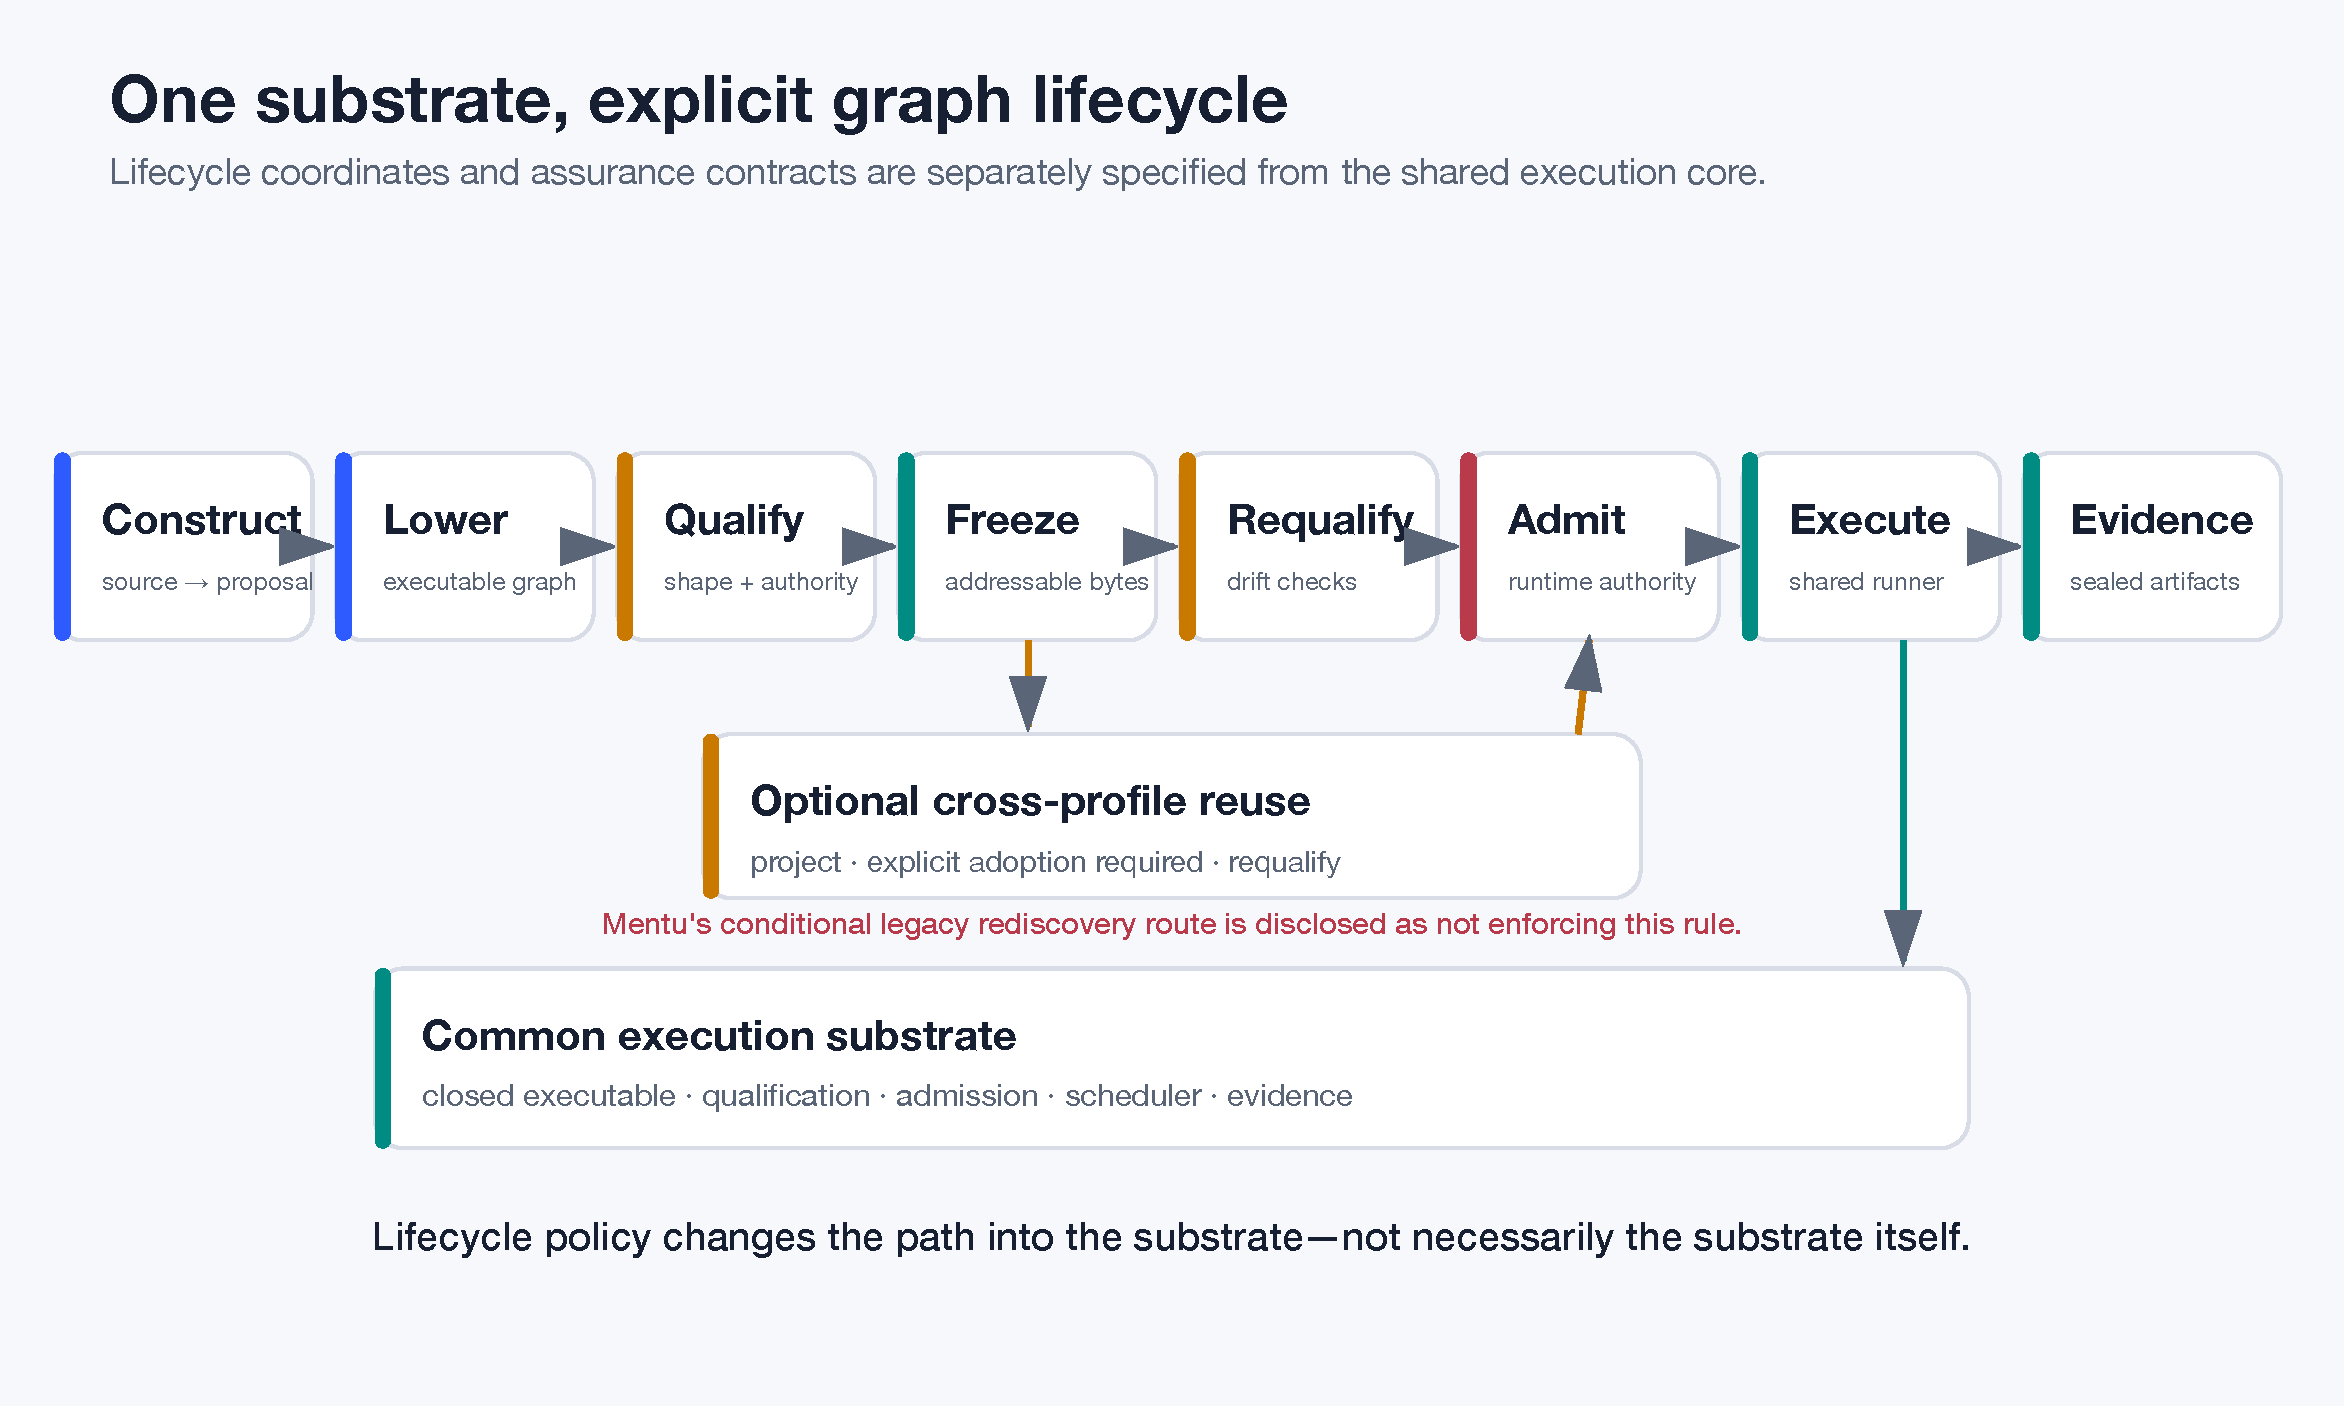
\includegraphics[width=\linewidth]{figs/fig1-lifecycle.pdf}%
  }{%
    \FigurePanel{Unified lifecycle and common substrate}{%
      Author $\rightarrow$ construct $\rightarrow$ lower $\rightarrow$
      qualify $\rightarrow$ freeze $\rightarrow$ requalify $\rightarrow$
      admit $\rightarrow$ execute $\rightarrow$ evidence.  Static, dynamic,
      and staged policies select different construction and freeze boundaries;
      admitted executions share the substrate.%
    }%
  }
  \caption{The maximal graph lifecycle.  Policy changes occur before
  execution; the common substrate executes the qualified graph, while
  authority-entry convergence is evaluated separately.}
  \label{fig:lifecycle}
\end{figure}

\subsection*{Binding schema, artifact header, and non-equivalent identities}

Let the binding schema selected by the external pin be
\[
\beta_{\bar\nu_\beta}
=
(D_\beta,p_\beta,
\{\approx_f\}_{f\in D_\beta},\mathsf{type}).
\]
Here \(D_\beta\) inventories declared bindable fields independently of the
artifact and receipt encoders, while
\[
p_\beta:D_\beta\rightarrow\{\nu,\chi,\eta\},
\qquad
F_k^\beta=p_\beta^{-1}(k),
\qquad
D_\beta=F_\nu^\beta\mathbin{\dot\cup}
F_\chi^\beta\mathbin{\dot\cup}F_\eta^\beta.
\]
The exact-match identity-header class is
\(F_\nu^\beta=\{\nu_L,\nu_C,\nu_\beta\}\);
\(F_\chi^\beta\) contains payload fields and \(F_\eta^\beta\) contains
residual environment fields bound at admission. Superscripts are omitted when
\(\beta\) is fixed. Field types and per-field equivalence relations are
declared independently of the canonicalizer. The mandatory payload core is
\[
  \{V,E,\lambda,\kappa,\sigma_g,P\}\subseteq F_\chi.
\]

Placement uses separate substitution domains. Intrinsic executable semantics
\[
\mathcal I_\rho(\chi)
=\bigl(\mathcal L_\rho(\chi),K_\rho^\chi\bigr)
\]
contains the unfiltered language of control, proposal, verification, and
attempted-effect traces and any executable-bound transition law. Holding
\(\rho\) fixed, a lowering-time field whose well-typed one-field payload
substitution changes \(\mathcal I_\rho\) belongs in \(F_\chi\). Node identity,
behavior, contracts, precedence, graph-declared scheduling, and
executable-bound policy are mandatory instances.

Authority-conditioned semantics is a different object:
\[
\mathcal A_\rho(\chi,\eta)
=\bigl(\operatorname{Admissible}_\rho(\chi,\eta),
\mathcal L_\rho^{\mathrm{allowed}}(\chi,\eta),
K_\rho^{\mathrm{run}}(\chi,\eta)\bigr).
\]
Holding \((\rho,\chi)\) fixed, an admission-time field whose well-typed
one-field environment substitution changes that decision or allowed trace
projection, or the context-resolved execution law, belongs in \(F_\eta\); it
does not redefine
\(\mathcal I_\rho(\chi)\). Requested effect scope is a payload contract.
Granted permission, credentials, sandbox/approval posture, and independently
resolved routes are residual environment facts. A model/backend selector is
\(F_\chi\) only when frozen in the executable and thus part of
\(K_\rho^\chi\); a route resolved independently at admission is a distinct
\(F_\eta\) fact. Provider sampling after admission is \(\xi\). Lowerer,
canonicalizer, and schema versions remain \(F_\nu\) provenance. An omitted,
bindable fact cannot be relabeled exogenous to protect the schema.

These placement predicates are denotational; the paper does not assume that
equality of arbitrary stochastic trace languages is decidable. Operational
tests instead declare a finite observation profile

\[
\omega=(h,\pi_{\omega},\zeta),
\]

where \(h\) is a transition horizon, \(\pi_{\omega}\) is an event projection
(subscripted to keep it distinct from the lifecycle policy vector \(\pi\);
finding BR9-004 of the v0.9.9-r6 blind review), and
\(\zeta\) is a reproducible choice harness. A controlled substitution that
changes the resulting observation is a bounded witness against equivalence.
An unchanged finite observation is only non-falsification under that
\(\omega\); it does not prove denotational equality or causal inertness.

The v0.9.9-r6 blind review observed (finding BR9-001) that a profile left to
the author and absent from the published evidence vector makes
non-falsification unearned: a projection too coarse to distinguish anything
yields it for free. The concrete profile is therefore published. Every
non-falsification this paper reports was observed under one profile,
\(\omega_{0}\): the horizon \(h\) is the complete archived run record of each
reported run, from admission through terminal state, untruncated; the event
projection \(\pi_{\omega}\) is the canonicalizer's identity-bearing field
projection at the pinned \(F_\nu\) versions; and the choice harness \(\zeta\)
is the committed reproduction wrapper at its archived commit, executed
against byte-fixed archives with no live provider sampling, so \(\xi\) is not
exercised. \(\omega_{0}\) is carried as the eighth component of \(\Gamma_E\),
and every reported non-falsification is paired with the positive detection
controls of Section~8 — three of three historical disposable-copy mutations
detected, one of one current-Core admission-drift control detected — so a
profile that detects nothing is distinguishable from a genuine equivalence:
under \(\omega_{0}\) the detectors fire on seeded differences and do not fire
on the reported substitutions. An adequacy condition constraining
\(\pi_{\omega}\) in general remains open and unclaimed.

Effect-semantic equivalence is explicit:
\[
\chi_1\equiv_\beta \chi_2
\Longleftrightarrow
\forall f\in F_\chi,\;
\operatorname{value}_{\chi_1}(f)\approx_f
\operatorname{value}_{\chi_2}(f).
\]

The per-field relations also carry a trace-soundness obligation for every
substrate contract \(\rho\) claimed by the profile:
\[
\operatorname{TraceSound}_{\rho}(\beta)
\Longleftrightarrow
\forall\chi_1,\chi_2,\quad
\chi_1\equiv_\beta\chi_2
\Rightarrow
\mathcal I_\rho(\chi_1)\equiv\mathcal I_\rho(\chi_2).
\]
Finite observations can falsify this obligation but cannot certify it
universally. This keeps a coarse field-equivalence rule from silently erasing a
trace-distinguishing payload change while leaving byte canonicalization
formally conforming to that coarse rule.
Residual-environment equivalence is defined independently:
\[
\eta_1\equiv_{\eta,\beta}\eta_2
\Longleftrightarrow
\forall f\in F_\eta,\;
\operatorname{value}_{\eta_1}(f)\approx_f
\operatorname{value}_{\eta_2}(f).
\]
It carries the parallel environment/authority obligation
\[
\operatorname{AuthoritySound}_{\rho,\chi}(\beta)
\Longleftrightarrow
\forall\eta_1,\eta_2,\quad
\eta_1\equiv_{\eta,\beta}\eta_2
\Rightarrow
\mathcal A_\rho(\chi,\eta_1)=\mathcal A_\rho(\chi,\eta_2).
\]
A coarse relation may therefore not erase a change in admission, allowed
traces, or the context-resolved execution law. A controlled
\(\operatorname{Obs}^{A}_{\rho,\omega}\) difference falsifies authority
soundness under the declared profile; finite equality is only
non-falsification, never a universal certificate. Environment canonicalization
must preserve the declared relation rather than silently substitute pathname
or serialization equality.

The accepted identity profile \(\bar\nu\) is selected outside the artifact;
the header does not recursively select the function that interprets it.
Before canonicalization or qualification, the strict model checks
\[
\operatorname{HeaderOK}_{\bar\nu}(x)
\Longleftrightarrow \nu(x)=\bar\nu.
\]
A mismatch refuses before canonicalization and before host effects. Only then
does the externally selected canonicalizer consume \(\chi\). It conforms to
\(\beta_{\bar\nu_\beta}\) only when both directions hold:
\[
\operatorname{canon}_{\bar\nu_C,\beta}(\chi_1)
=\operatorname{canon}_{\bar\nu_C,\beta}(\chi_2)
\Longleftrightarrow \chi_1\equiv_\beta\chi_2.
\]
Canonical artifact bytes separately frame a fixed header encoding and the
canonical payload:
\[
b_{\bar\nu,\beta}(x)
=\operatorname{frame}\!\left(
\operatorname{canonHeader}(\nu(x)),
\operatorname{canon}_{\bar\nu_C,\beta}(\chi)
\right),
\qquad \operatorname{HeaderOK}_{\bar\nu}(x).
\]
Thus a header change creates a new artifact identity without being mislabeled
as a trace-semantic mutation. In the \mentu{} instantiations and paper tools,
\(H\) is full-length SHA-256 and executable identity is
\[
  h_x=\operatorname{SHA256}(b_{\bar\nu,\beta}(x)).
\]
For run \(j\), define the residual binding after requalification and concrete
context selection as
\[
\eta_{\beta,j}:=
\operatorname{bind}_{F_\eta^\beta}
(s_j,a_j,q_{\mathrm{rq},j},c_j).
\]
Environment identity is the separate binding
\(h_{\eta,j}=\operatorname{SHA256}(
\operatorname{canon}_{\eta,\beta}(\eta_{\beta,j}))\), when an aggregate is
computed. Truncated hexadecimal strings in figures are labels, never
identities.

Two tests must remain separate. For admitted run \(j\), let \(U_j\) inventory
identity-bearing field names actually recovered from the executable and
receipt, and let
\(O_j\subseteq U_j\times\{\nu,\chi,\eta\}\) record their observed placement
without copying \(p_\beta\). \emph{Declared binding closure} requires
\[
U_j=D_\beta,\qquad
\forall f\in D_\beta,\quad
\{k:(f,k)\in O_j\}=\{p_\beta(f)\}.
\]
This compares an independent declared inventory with observed encoding and
requires complete, unique placement; it is not merely the declared partition
identity above. \emph{Schema adequacy} asks whether a bindable causal fact was
omitted. An omission probe holds \(x\) and declared \(\eta\) fixed, varies one
undeclared candidate fact such as execution-model identity, permission
posture, clock, or locale, and observes whether admission, the allowed trace
projection, or the context-resolved execution law changes. A positive witness
is a schema defect and bars an adequacy claim under that \(\beta\).

Before admission, the schema itself must also be well formed: \(p_\beta\) is
total and typed on \(D_\beta\); its three inverse images are pairwise disjoint;
every non-header identity field has exactly one declared semantic-class
assignment with an addressable analytic or external justification; and the
independently enumerated identity-bearing names emitted by executable and
receipt encoders equal \(D_\beta\). The mechanical gate checks declaration
presence, uniqueness, placement, and encoder closure; it is not a semantic
oracle. Unassigned names, names without a declared semantic class, dual-domain,
undeclared-emitted, declared-but-unemitted, and multiply placed names cause
refusal. Trace soundness, authority soundness, and open-world adequacy remain
semantic obligations that finite witnesses can falsify but cannot prove.

RFC~8785 specifies a canonical JSON serialization for stable hashing, including
primitive serialization and deterministic property ordering
\cite{Rundgren2020JCS}. The model's canonicalizer must state whether it conforms
to that baseline or deliberately differs. Its declared semantic equivalence,
path/content aliases, field placement, and artifact framing are domain
extensions; RFC~8785 does not establish them. Canonicalizer evidence likewise needs both directions: well-typed semantic
mutations must produce distinct canonical bytes, while equivalent encodings
such as key ordering, normalized numbers, and declared path equivalents must
converge. An \(F_\eta\)-only change must leave \(h_x\) unchanged while changing
the environment binding or admission decision. The present evidence does not
establish complete schema adequacy or full biconditional canonicalizer
conformance. Neither the historical C30 pin nor the current Core pin exercises
a \(\operatorname{HeaderOK}_{\bar\nu}\) mismatch-before-effects fixture, so
header refusal remains a specification obligation rather than an observed pass
at either pin.

In the historical C30 \mentu{} path at \code{\MentuCommitShort}, the full
\code{SequenceDefinition} binds nodes and \code{dependsOn} relations, while
the frozen backend/model selector, other executable-bound policy, and lowerer
version are also bound by the executable artifact. Under the refined model,
the graph and executable-bound policy fields belong to \(F_\chi\), while the
lowerer version belongs to \(F_\nu\). Repository and discovery state, granted
authority, qualification state, resolved credential/endpoint posture, and
concrete admission context remain in \(F_\eta\). This field-placement example
interprets the historical pilot; it is not projected forward onto the current
Core definition.

Even if both identities match, an agent node may be stochastic.  Output
reproducibility is therefore a property of observations from
\[
  Y \sim \mathcal{D}(\,\cdot \mid x,\eta,\xi\,),
\]
where \(\xi\) includes model sampling, remote service behavior, and other
uncontrolled state. Semantic judgment has two distinct targets:
\(\operatorname{PlanAdequate}(x,o)\) asks whether the executable expresses an
appropriate course of action for the objective, while
\(\operatorname{OutcomeCorrect}(y,o)\) asks whether an observed outcome
satisfies it. Graph identity, environment identity, output reproducibility,
plan adequacy, and outcome correctness require different evidence and are
never substituted for one another in this paper.

\subsection*{Projection is not adoption}

A frozen executable may be projected into a persistent source form \(p\) for
evidence or reuse. Projection parity requires that pinned lowering reproduce
the executable identity bound by \(z\); it does not grant authority. If \(p\)
later enters a different assurance contract \(\psi_t\), the transition is
explicit:
\[
\operatorname{Project}(z)\rightarrow p,\qquad
\operatorname{Adopt}(p,\psi_t,a,s)\rightarrow(x_t,q_t)\mid\operatorname{refuse}.
\]
Adoption names the target contract, re-lowers or loads the artifact, qualifies
it, and requires that contract's admission transition before effects.
Discoverability through another parser or command is not adoption. This rule
keeps authoring origin out of runtime authority while preventing parseable
bytes from silently inheriting the weakest available entry path.

\section{Lifecycle policies}

The C30 policy vector is
\[
  \pi=(\tau,\phi,\mu,\rho),
\]
where \(\tau\) is construction time, \(\phi\) is the freeze boundary,
\(\mu\) is authoring method, and \(\rho\) is execution substrate.  Let
\[
  \Omega \subseteq T \times \Phi \times \mathcal M \times R
\]
be the feasible policy region.  The coordinates are separately specified:
changing one does not redefine the others.  This is a separability claim over
\(\Omega\), not a claim that every Cartesian combination is feasible,
independent in a statistical sense, or free of engineering constraints.  The
named modes are reference configurations, not an exhaustive taxonomy.
The normative coordinate vocabulary is:
\(\tau\in\{\text{pre-task},\text{task-time}\}\);
\(\phi\in\{\text{continuous},\text{addressable}\}\);
\(\mu\) names the source-production method; and \(\rho\) names the
runner-and-scheduler substrate whose execution semantics are being compared.
The plan container \(z\) is the addressable lifecycle record used by
addressable-\(\phi\) policies; \(z\) binds \(x\) but is not synonymous with it.

An entry policy also has an assurance contract
\(\psi_p=(\mathcal Q_p,\mathcal A_p,\mathcal E_p)\), comprising its
qualification regime, admission transition, and evidence contract.  This is
not a fifth C30 treatment axis.  It makes explicit that
\(\rho_p=\rho_q\) does not imply \(\psi_p=\psi_q\): policies can share
execution semantics while retaining different assurance contracts.
Here \(\psi\) is an author-declared runtime contract, not an independently
evaluated security profile, protection profile, or certification level.

\begin{table}[htbp]
\centering
\small
\begin{tabularx}{\linewidth}{@{}p{0.10\linewidth}YYYY@{}}
\toprule
Mode & Construction time & Freeze boundary & Authoring method & Execution substrate \\
\midrule
S & Before task invocation & Addressable source before invocation & Method \(\mu_S\) & Shared graph substrate (model) \\
D & At task invocation & Continuous construction-to-execution invocation & Method \(\mu_D\) & Shared graph substrate (model) \\
H-direct & At task invocation & Addressable plan before a later execution invocation & Direct planner & Shared graph substrate (model) \\
H-scaffold & At task invocation & Addressable plan before a later execution invocation & Scaffold authoring method & Shared graph substrate (model) \\
\bottomrule
\end{tabularx}
\caption{Reference policies as configurations of separately specified
lifecycle coordinates in the feasible region \(\Omega\). ``Shared'' is a model
parameter and an implementation question, not a universal fact about all
systems.}
\label{tab:policies}
\end{table}

These four points do not empirically demonstrate independent variation of all
coordinates: \(\rho\) is held constant, and the observed \(\tau,\phi\) values
are only partially crossed. Separability is therefore a specification claim
about how a configuration is described, not an identified causal effect or a
claim that the reference points span \(\Omega\).

\begin{figure}[htbp]
  \centering
  \IfFileExists{figs/fig2-policy-axes.pdf}{%
    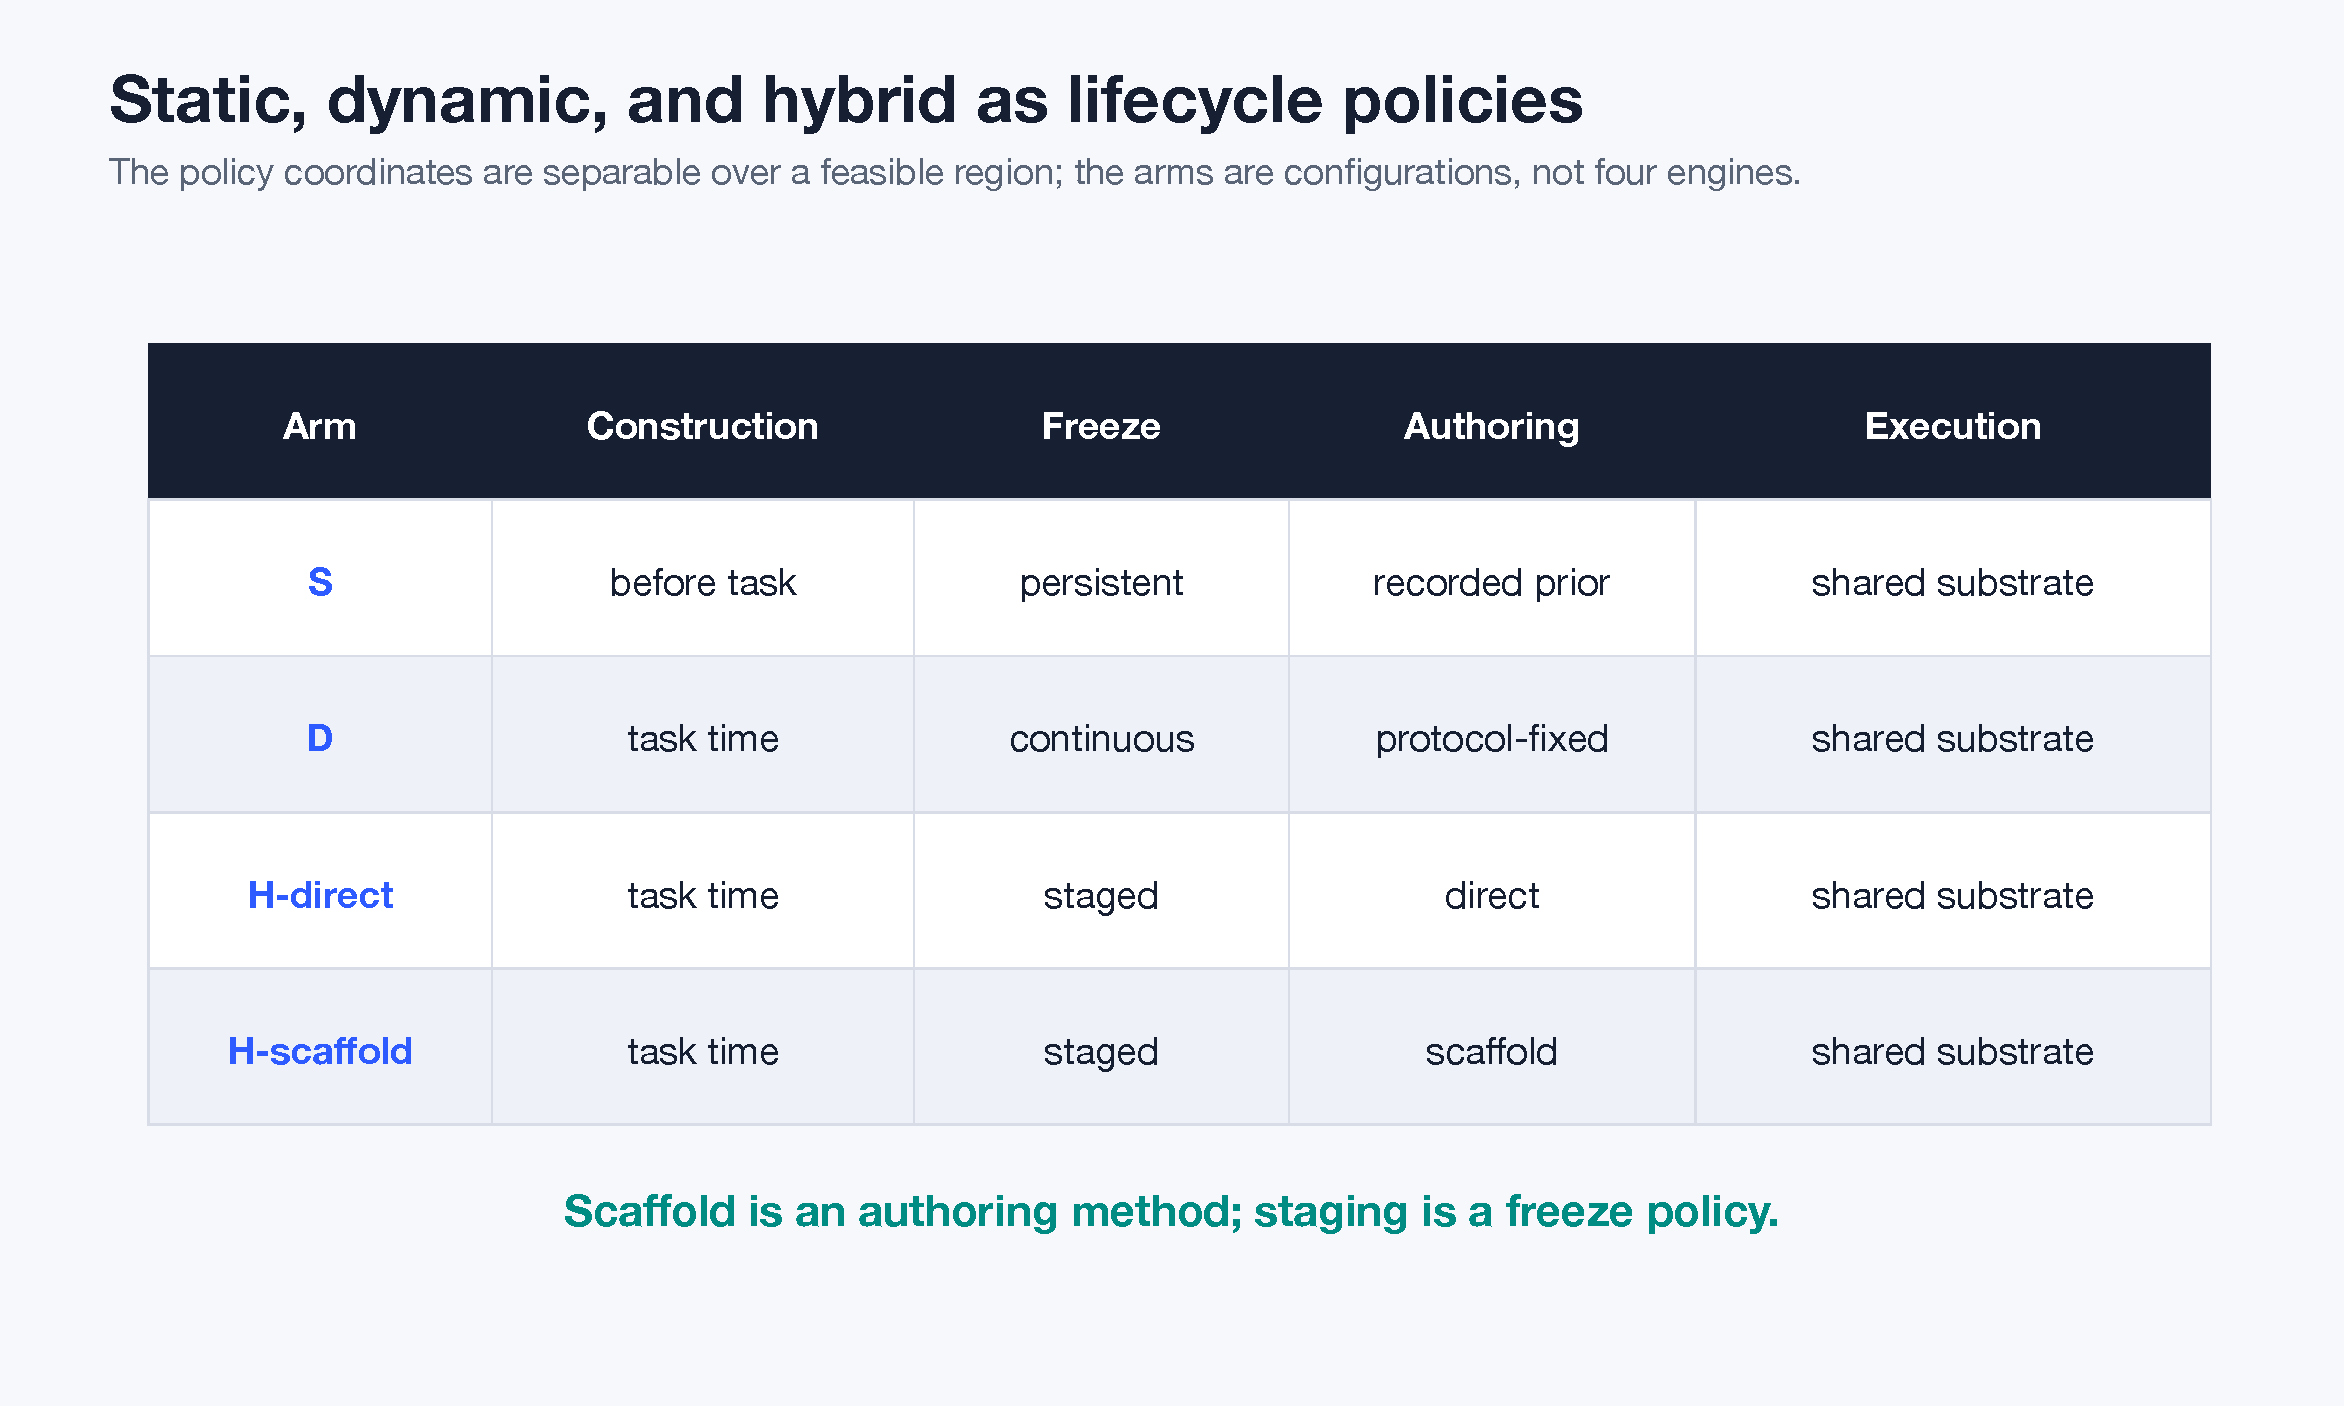
\includegraphics[width=\linewidth]{figs/fig2-policy-axes.pdf}%
  }{%
    \FigurePanel{Policy-axis matrix}{%
      S: pre-task construction and persistent freeze.  D: task-time
      construction and continuous plan--run invocation.  H-direct and
      H-scaffold: task-time construction followed by an addressable freeze;
      they differ only in authoring method.  All reference modes target one
      execution substrate.%
    }%
  }
  \caption{S, D, H-direct, and H-scaffold occupy points in one policy space.
The labels do not define separate runner implementations.}
  \label{fig:policy-axes}
\end{figure}

Two consequences follow from the factorization.  First, ``scaffold'' is not a
runtime kind. Here it names an authoring method, not the broader model-and-tool
harness also called a scaffold in agent literature. If it changes only
\(\mu\), then a scaffolded candidate must
satisfy the same lowering, qualification, admission, and execution contracts
as a directly authored candidate.  Second, a static source need not have been
written by a human, and a dynamically constructed source need not execute
immediately.  Provenance, timing, freezing, and execution are separable.

The word \emph{hybrid} remains useful only when its boundary is named.  Here it
means dynamic construction followed by an explicit, addressable freeze and a
later requalification-and-execution invocation.  It does not mean two runtimes,
weaker contracts, or continued planner authority while the frozen epoch runs.

\subsection*{Four separate evaluation decisions}

The model does not use one word, ``implemented,'' for four different
questions. First, an \emph{author-checked architectural instantiation} requires
an origin-neutral executable type, one declared scheduler contract, and
mapped construction or loading boundaries that can target them. Committed
source and named engineering tests must support that mapping. This label
denotes an author-performed check, not an independent audit or canonical
reference status.

Second, \emph{executed cross-origin parity} is stronger: at least two feasible
lifecycle policies must lower or load equivalent fixtures, enter the same
runner, receive the same node-dispatch and graph-declared scheduling
semantics, and show that origin-specific metadata does not silently alter
those semantics. The evaluation must follow and execute both traces; a source
definition or unexecuted fixture is insufficient.

Third, full staged binding/admission conformance requires I1--I6 under fixed
versions, including exercised I4 drift categories and complete I5
declared-closure and mandatory-field mutation fixtures. Shared machinery alone
is insufficient.

Fourth, logical safety is reported separately from operational evidence
adequacy. Implications can pass vacuously in a runtime that refuses everything.
We therefore report
\[
\Gamma_E=(n_{\mathrm{recorded\ host\mbox{-}boundary\ runs}},n_{\mathrm{distinct}\ x},
n_{\mathrm{projection}},|J_{\bar\nu,\beta,f}|,
n_{\mathrm{header\ refusal}},\mathcal D_{\mathrm{I4}},
\mathcal M_{\mathrm{I5}},\omega).
\]
The eighth component publishes the concrete observation profile under which
the reported non-falsifications were observed (Section~3, \(\omega_{0}\)),
so the strength of every equivalence statement is inspectable rather than
implicit. \(\Gamma_E\) is published for the historical population only, by
design at this candidate: current-Core engineering tests are reported outside
this vector, and any future current-pin claim must carry its own
\(\Gamma_E\) (finding BR9-005).
At least one admitted run with recorded host-boundary activity is required for
instrumented non-vacuity; this count is not proof that every semantic effect
was observed. A
cross-input identity claim requires at least two executable identities; I3
requires a projection; I1 must expose its eligible population; and every
claimed header, I4, or I5 category requires a seeded or observed witness. The
historical pilot is non-vacuous for I1--I3 but has no header-refusal fixture, I4
challenge, or complete I5 matrix. Paper-local detector controls and
current Core tests are separate evidence, not retroactive pilot observations.

\section{Qualification, freeze, admission, and execution invariants}

The lifecycle becomes operational only when its transitions have testable
obligations. The author check of the pinned commit supports an architectural
instantiation for the named strict-DAG Core profile. Current tests
exercise origin-neutral lowering, an admitted vertical slice, saved-plan
execution, canonicalization, and drift refusal, but they do not execute an
ordinary static recipe and a generated graph through one Core admission route.
Product-wide executed cross-origin parity is therefore not claimed. Full
staged-protocol conformance additionally requires I1--I6 under fixed versions,
exercised I4 drift classes, and a complete I5 fixture matrix. C30 tests only a
subset of that stronger protocol at its separate historical pin.

\paragraph{I1---staged executable identity.}
Fix \(\bar\nu\), \(\beta=\beta_{\bar\nu_\beta}\), and receipt field
\(f=\operatorname{executableId}\). Let
\(J_{\bar\nu,\beta,f}\) contain the
staged invocations for which requalification succeeds, no bound-field drift is
detected, and admission returns a pre-effect receipt exposing \(f\). For every
\(j\in J_{\bar\nu,\beta,f}\):
\[
\operatorname{SHA256}(b_{\bar\nu,\beta}(x_{\mathrm{inspect},j}))
=\operatorname{SHA256}(b_{\bar\nu,\beta}(x_{\mathrm{rq},j}))
=r_j.f.
\]
If the saved artifact stores a candidate rather than only an executable,
re-lowering must reproduce the saved executable bytes under the pinned lowerer
and canonicalizer.  The pilot instantiates this condition only for the
\mentu{} v1 lowerer, canonicalizer, commit, and receipt field named in the
author source check. The identity ratio is conditional on reaching \(J\), so every
report must also publish the attempted, requalification-refused,
admission-refused, admitted, and identity-matched counts. It is not a pipeline
success rate.

\paragraph{I2---no execution-time graph planning.}
Let \(J_{\mathrm{saved}}\) contain invocations registered before any run
telemetry as entering through the saved-plan requalify-and-admit route with an
existing addressable plan. Membership is fixed by that entry route, not by the
later dispatch outcome. The invariant is
\[
\forall j\in J_{\mathrm{saved}},\qquad
N_{\operatorname{Construct},j}^{exec}=0.
\]
A model call that implements an admitted node is execution, not graph
planning; the two lanes must be separately classified. An observed
graph-construction dispatch is an I2 failure retained in
\(J_{\mathrm{saved}}\), not grounds for post-outcome reclassification.

\paragraph{I3---persistent projection parity.}
When a generated executable is materialized as a persistent recipe projection,
their canonical executable identities must be equal.  This establishes parity
for the materialized artifact; it does not move all persistent recipes through
the generated path or prove global admission convergence. A parity pass is the
conjunction of lossless projection and deterministic pinned lowering; without
a separate lowerer-determinism control it does not identify which component
would explain a failure.

\paragraph{I4---drift refusal before effect.}
Executable identity does not waive current-state checks.  Requalification must
bind the frozen graph to the current \(\eta_1\), and drift outside the admitted
policy must refuse before host dispatch and target-path change.  Requalification
may reject exact bytes; rejection preserves, rather than contradicts, I1. C30
prospectively specifies this invariant, but the pilot deliberately challenged
zero drift classes. Its source mapping and prospective specification are not
empirical drift-test evidence.

\paragraph{I5---declared binding closure.}
For every admitted run \(j\), the independently declared inventory and
placement map must agree with the observed executable/receipt inventory and
placement relation:
\[
U_j=D_\beta,\qquad
\forall f\in D_\beta,\quad
\{k:(f,k)\in O_j\}=\{p_\beta(f)\}.
\]
The executable binds every field assigned to \(F_\nu\) and \(F_\chi\); the
receipt binds every declared \(F_\eta\) constituent or an aggregate identity
with declared equality semantics, a schema-versioned ordered constituent
inventory, and addressable evidence from which the aggregate can be recomputed.
An opaque aggregate cannot satisfy \(U_j=D_\beta\). An extra,
missing, duplicated, or misplaced identity-bearing field, a header/pin
mismatch, or an unbound declared environmental constituent causes refusal
before effect. A failed payload inequivalence, equivalence,
partition-isolation, or header fixture makes the relevant binding or
canonicalization claim nonconforming under that \(\beta\).

The C30 pilot observes selected executable and receipt bindings, but it does
not compare an independent complete \(D_\beta\) inventory with \(U_j\), and it
does not exercise a complete mandatory-field mutation suite. It therefore does
not establish full declared closure or biconditional canonicalizer
conformance. Neither the C30 pin nor the current Core pin exercises
\(\operatorname{HeaderOK}_{\bar\nu}\) mismatch refusal. Schema adequacy is a
separate open-world property requiring omission probes over plausible
undeclared bindable facts; neither declared closure nor a conforming
canonicalizer establishes it.

\paragraph{D1---authoring/authority non-implication.}
A candidate, qualified candidate, and frozen plan have no implied effect
authority.  Admission produces a bounded authority state, and changing
\(\mu\) cannot change that state when the executable, qualification result,
external authority envelope, and bound runtime context are equal.  If an
explicit qualification, authority, or runtime contract names the profile,
the authoring method becomes an authority-bearing policy input and the
implication no longer applies. This is a construct boundary, not an empirical
invariant: scaffold describes construction unless a named authority contract
says otherwise.

\paragraph{I6---evidence integrity.}
For this model the run record must bind six things: the executable, authority
envelope, qualification result, concrete runtime context, run identity, and
artifact manifest.  This is a closed mandatory set.  Every manifest file
digest and its derived aggregate bundle digest must recompute. I5 establishes
field placement; I6 establishes that the receipt, run identity, and artifact
manifest survive as addressable evidence. The pilot
verified receipt fields and manifest digests but did not compute a standalone
aggregate \(h_\eta\).
At the current \mentu{} pin, the concrete runtime context is not an unnamed
placeholder: it includes the run and workspace roots, transfer mode, locks and
baselines, Git and selected-read-set digests, dependencies and variables,
the resolved backend/model route (distinct from any executable-frozen
selector), auth, endpoint, permission, sandbox, approval, MCP, primitive and
adapter identities, engine version, qualification/runtime state digests, and
outer-call/gate posture. The executed drift control perturbs the declared
\code{runtimeStateDigest}; it is an \(F_\eta\)-side admission check, not an
executable-field mutation.
Evidence is a product of execution, not a transcript substituted for an
addressable artifact.

\paragraph{D2---semantic non-implication.}
Mechanical qualification is sound only relative to its declared checks.
Passing schema, dependency, footprint, budget, or verification predicates does
not prove plan adequacy or outcome correctness. In particular:
\[
\bigwedge_{k=1}^{6}I_k
\not\Rightarrow \operatorname{PlanAdequate}(x,o),
\qquad
\bigwedge_{k=1}^{6}I_k
\not\Rightarrow \operatorname{OutcomeCorrect}(y,o).
\]
D1 is excluded because it is an analytic construct boundary, not an empirical
protocol invariant.

\subsection*{Scope theorem: runtime replanning}

Let receipt \(r_0\) admit \(x_0\), whose graph-semantic core is \(G_0\). After
execution begins, suppose a planner changes a node, dependency, behavior
binding, node contract, or graph-declared scheduling transition to produce
\(x_{\mathrm{succ}}\). The narrow identity lemma has the explicit antecedent
\[
\chi_{\mathrm{succ}}\not\equiv_\beta\chi_0.
\]
Given that antecedent and a canonicalizer conforming to \(\beta\):
\[
  b_{\bar\nu,\beta}(x_0)
  \ne b_{\bar\nu,\beta}(x_{\mathrm{succ}}).
\]
Under the stated collision-resistance assumption,
\[
  \operatorname{SHA256}(b(x_0))
  \ne \operatorname{SHA256}(b(x_{\mathrm{succ}}))
  \quad\Longrightarrow\quad
  r_0 \text{ does not bind }x_{\mathrm{succ}}
\]
except in the digest-collision case. Dispatching \(x_{\mathrm{succ}}\) under
\(r_0\) violates the non-mutating admission binding. A same-byte
trace-relevant mutation exposes a trace-unsound \(\beta\), a field-placement
defect, or canonicalizer nonconformance; it is not an identity distinction. A
distinct-byte same-digest observation challenges the digest assumption. A
scheduler-build change rather than graph-declared scheduling changes the bound
environment identity or causes refusal.

The stronger semantic corollary may derive the narrow antecedent only when
\[
\mathcal I_\rho(\chi_{\mathrm{succ}})\not\equiv
\mathcal I_\rho(\chi_0)
\quad\land\quad
\operatorname{TraceSound}_\rho(\beta).
\]
A coarse relation that treats \(A\!\to\!B\) and \(B\!\to\!A\) as equivalent
because they share endpoint names can preserve canonical bytes while reversing
observable order. That is a counterexample to trace soundness of the schema,
not evidence that identity distinguished the mutation. A finite
\(\operatorname{Obs}^{I}_{\rho,\omega}\) difference is a bounded witness, not a
universal certificate.

An \emph{admission-scoped graph epoch} is the interval governed by one receipt
and executable identity. The term borrows the fencing intuition of a
generation change but makes no claim about distributed consensus, leader
election, or a product-wide epoch counter.

There are two coherent alternatives. The system can close epoch \(e_0\),
construct and qualify \(G_1\), and issue a new admission for epoch \(e_1\); or
it can define an adaptive runtime in which the planner and its allowed
transition relation are themselves part of the admitted executable semantics.
The latter may keep a fixed outer graph while producing data-dependent work,
but it is not execution of the same frozen inner topology. Runtime replanning
that changes graph structure or scheduling semantics without either treatment
is outside the frozen-epoch protocol population. An interpreted surface
that claims neither a complete graph nor an admitted meta-runtime identity is
a third honest classification. This is a scope boundary, not an empirical
counterexample or falsifier of the model. Its value is discriminant: it states
which object must carry authority when topology remains adaptive. A fixed outer
behavior tree is one established way to represent data-dependent control
without silently changing the admitted inner object
\cite{Colledanchise2017BehaviorTrees}.

\section{Mentu as an Author-Checked Architectural Instantiation}

The evidence is intentionally split across two source epochs. Historical C30
observations and their original source corroboration remain pinned to
\code{\MentuCommitShort}. The current architecture mapping is pinned
independently to \code{\MentuCurrentCommitShort}. The later Core extraction is
not inferred backward into the pilot.

At the current epoch, \mentu{} is the paper's author-checked architectural
instantiation of the strict-DAG admitted Agent Graph Runtime profile.
``Author-checked'' means an author-proposed model-to-system mapping checked
against committed source and named engineering tests executed by the
author-side reproduction harness. It is not an independent audit, external
certification, canonical reference status, a product-wide uniformity claim, or
a comparative rank.

\paragraph{An extracted admitted graph Core with a public API.}
\code{MentuExecutionGraphCore} owns the closed
\code{ExecutionGraph\allowbreak Definition}, lowering, canonicalization, qualification,
admission, activation evidence, lifecycle types, and
\code{ExecutionGraph\allowbreak Scheduler}. The checked
\code{MentuSequence\allowbreak Definition\allowbreak Adapter} is the boundary from MentuEngine's
general recipe schema to the admitted-only Core definition. MentuEngine retains
host effects, product integration, and presentation through adapters. Core
rejects unknown dependencies, self-dependencies, and cycles, so the admitted
profile is a strict DAG; neither the abstract model nor every Mentu surface is
therefore DAG-only.

\paragraph{One admitted scheduler, explicit compatibility profiles.}
Equivalent admitted definitions receive DAG validation, ready-set computation,
bounded parallelism, exclusivity, failure cascade, and circuit behavior from
the one Core scheduler. The engine's \code{StepScheduler} projects engine state
and bridges effectful node execution rather than defining a second DAG
scheduler. The prepared admitted path constructs the sole admitted
\code{SequenceRunner} only after Core admission and pre-host state validation.
Committed current-head test definitions cover persistent/generated origin
parity, admission drift refusal, and an admitted vertical slice. The
paper-local current-epoch verifier executes 13 named filters from an exact
Git archive with external build scratch and an isolated runtime home:
25 of 25 targeted tests pass. Coverage includes Core and engine
canonicalization, generated/persistent lowering parity, admission identity,
the admitted vertical slice, saved-plan exact execution, projection parity,
lifecycle ordering, pre-runner drift refusal, and the Engine--Core round trip.
These are author-side engineering tests, not independent black-box
replication or exhaustive schema conformance. None of the 13 filters exercises
\(\operatorname{HeaderOK}_{\bar\nu}\) mismatch refusal.

The current-epoch mapping follows generated and saved-plan prepared boundaries
to the same Core definition and scheduler, while its origin-parity fixture
compares equivalent generated and persistent lowerings. Historical C30 runner
evidence remains corroboration for its own pin and is not substituted for this
current-Core mapping. No test in this revision executes an ordinary static
recipe and a generated graph through one Core admission route, so
product-wide executed cross-origin parity remains unclaimed.

Mentu also retains deliberate compatibility profiles. Ordinary recipe dispatch
can use the raw \code{SequenceRunner} initializer with legacy authority, and
\code{mentu workflow run} uses the interpreted \code{WorkflowRunner}. Their
different assurance or execution contracts are profile boundaries, not
evidence that the admitted graph core is architecturally incomplete. They are
also not silently counted as conformance evidence for that Core.

The current committed-source census found \CurrentRecipeTypeCount{} persisted
recipe type cases, \CurrentSequenceRunnerConstructorCount{} direct production
\code{SequenceRunner} construction sites
(\CurrentLegacyRunnerConstructorCount{} raw and
\CurrentAdmittedRunnerConstructorCount{} admitted), and
\CurrentWorkflowRunnerConstructorCount{} direct \code{WorkflowRunner}
construction sites. These are exact lexical constructor counts, not a
denominator or percentage of every effectful Mentu entry point. The audit
classifies the graph-bearing roots it names and leaves other product operations
outside its population. A lexical census establishes where constructors are
written, not which are reachable or how often they execute: the
sole-admitted-runner statement it supports is a source-layout claim, and a
reachability-grade check (call-graph or runtime instrumentation over the
census population) is registered as future work, not claimed (finding
BR9-006 of the v0.9.9-r6 blind review).

\paragraph{Current projection-adoption boundary.}
The source audit found one concrete cross-profile transition boundary.
Persistent projection
writes a normal \code{recipe.json}, prompts, and parity evidence, but no
required-authority marker. If placed under ordinary recipe discovery, those
files can later be parsed by \code{mentu run} and reach legacy compatibility
authority without an explicit adoption transition. Recipe dispatch computes
effective auto behavior as CLI auto OR recipe auto. It nevertheless constructs
the raw \code{SequenceRunner} after any applicable precondition in all four
Boolean cells, and that initializer assigns legacy authority independently of
the effective-auto value:

\begin{table}[t]
\centering
\small
\begin{tabular}{@{}ccccc@{}}
\toprule
Recipe auto & CLI auto & Effective auto & Commit-record gate & Authority entry \\
\midrule
false & false & false & no  & legacy \\
false & true  & true  & no  & legacy \\
true  & false & true  & yes & legacy after gate \\
true  & true  & true  & no  & legacy \\
\bottomrule
\end{tabular}
\caption{Committed-source control-flow matrix for ordinary recipe dispatch.
The gate is a recipe-commit record existence check, not Core qualification or
admission. The matrix reports no operational traffic.}
\label{tab:recipe-dispatch-authority-matrix}
\end{table}

The unmodified generated projection occupies the recipe-auto-false row because
materialization adds no \code{auto\_mode} marker; CLI absence and explicit
false collapse to its false cell. The generated graph invocation itself enters
through the admitted route. The coherent alternate-contract transition is:
\[
\text{generated projection}
\rightarrow
\operatorname{Adopt}(\psi_t)
\rightarrow
\text{target qualification/admission}
\rightarrow
\text{execute}.
\]
Until Mentu enforces that transition, admitted authority must be described as
a property of the qualified-and-admitted invocation path, not an intrinsic
property of parseable projection bytes. This is a bounded cross-profile
adoption finding exposed by the model, not a verdict that the runtime
abstraction is missing. The source matrix establishes reachability and control
flow, not successful executions or use frequency in any cell.

\mentu{} makes the abstraction operational and inspectable: exploratory
construction can converge on a closed executable whose qualification,
admission, scheduling, activation evidence, and host boundary are explicit.
The current source establishes an admitted reference profile and named
compatibility surfaces. It does not establish global adoption enforcement,
exhaustive I5 mutation coverage, or comparative superiority.

\section{Historical C30 invariant-exercise method}

C30 prospectively committed the lifecycle axes and a matched four-arm study in
the author-controlled repository before the first pilot-evidence commit. The
protocol commit is \code{\CThirtyPreregCommitShort}; no external timestamp
anchor is claimed. The present analysis uses its smaller,
explicitly non-verdict-bearing mechanical invariant-exercise phase at the
historical \mentu{} source epoch \code{\MentuCommitShort}. It does not measure
the later Core extraction at \code{\MentuCurrentCommitShort}.

The pilot used \PilotObjectiveCount{} bounded documentation objective in
H-scaffold mode. A
task-time planner constructed a strict DAG under an external authority
envelope.  Plan-only execution emitted canonical plan bytes.  The operator
inspected the plan and materialized a persistent recipe projection and parity
record.  A later invocation loaded the exact saved plan, rebuilt and
requalified its executable against current state, admitted it, and invoked the
runner without another graph-planner call.  Read-only analysis then checked the
plan, persistent recipes and prompt files, parity records, requalified
admission bundles, receipts, call lanes, and sealed run manifests. For each
persistent projection it reconstructs the normalized definition, contracts,
effective policy, and canonical executable digest from source artifacts; the
stored parity record is a cross-check, not the derivation.
For each admitted execution it also rebuilds the requalified bundle identity
from the admitted definition, actual prompt bodies, bound variables, contracts,
and mechanically derived effective policy before comparing that digest with
the receipt; a copied stored digest cannot satisfy this check.
The planner-separation check has bounded, partly shared corroboration: the
execution records state the dispatch count; every sealed call-lane record is
bound to an admitted step activation and none is planner-classified; and a
lexical audit of the pinned \code{runPlanned} implementation finds no planner
emission. All three channels depend on recorded classification or one named
code path; they are not independent instrumentation. The result is therefore
zero \emph{recorded} planner dispatches, not proof that every possible
out-of-band planning path was observable.

\begin{center}
  \centering
  \IfFileExists{figs/fig3-runtime-paths.pdf}{%
    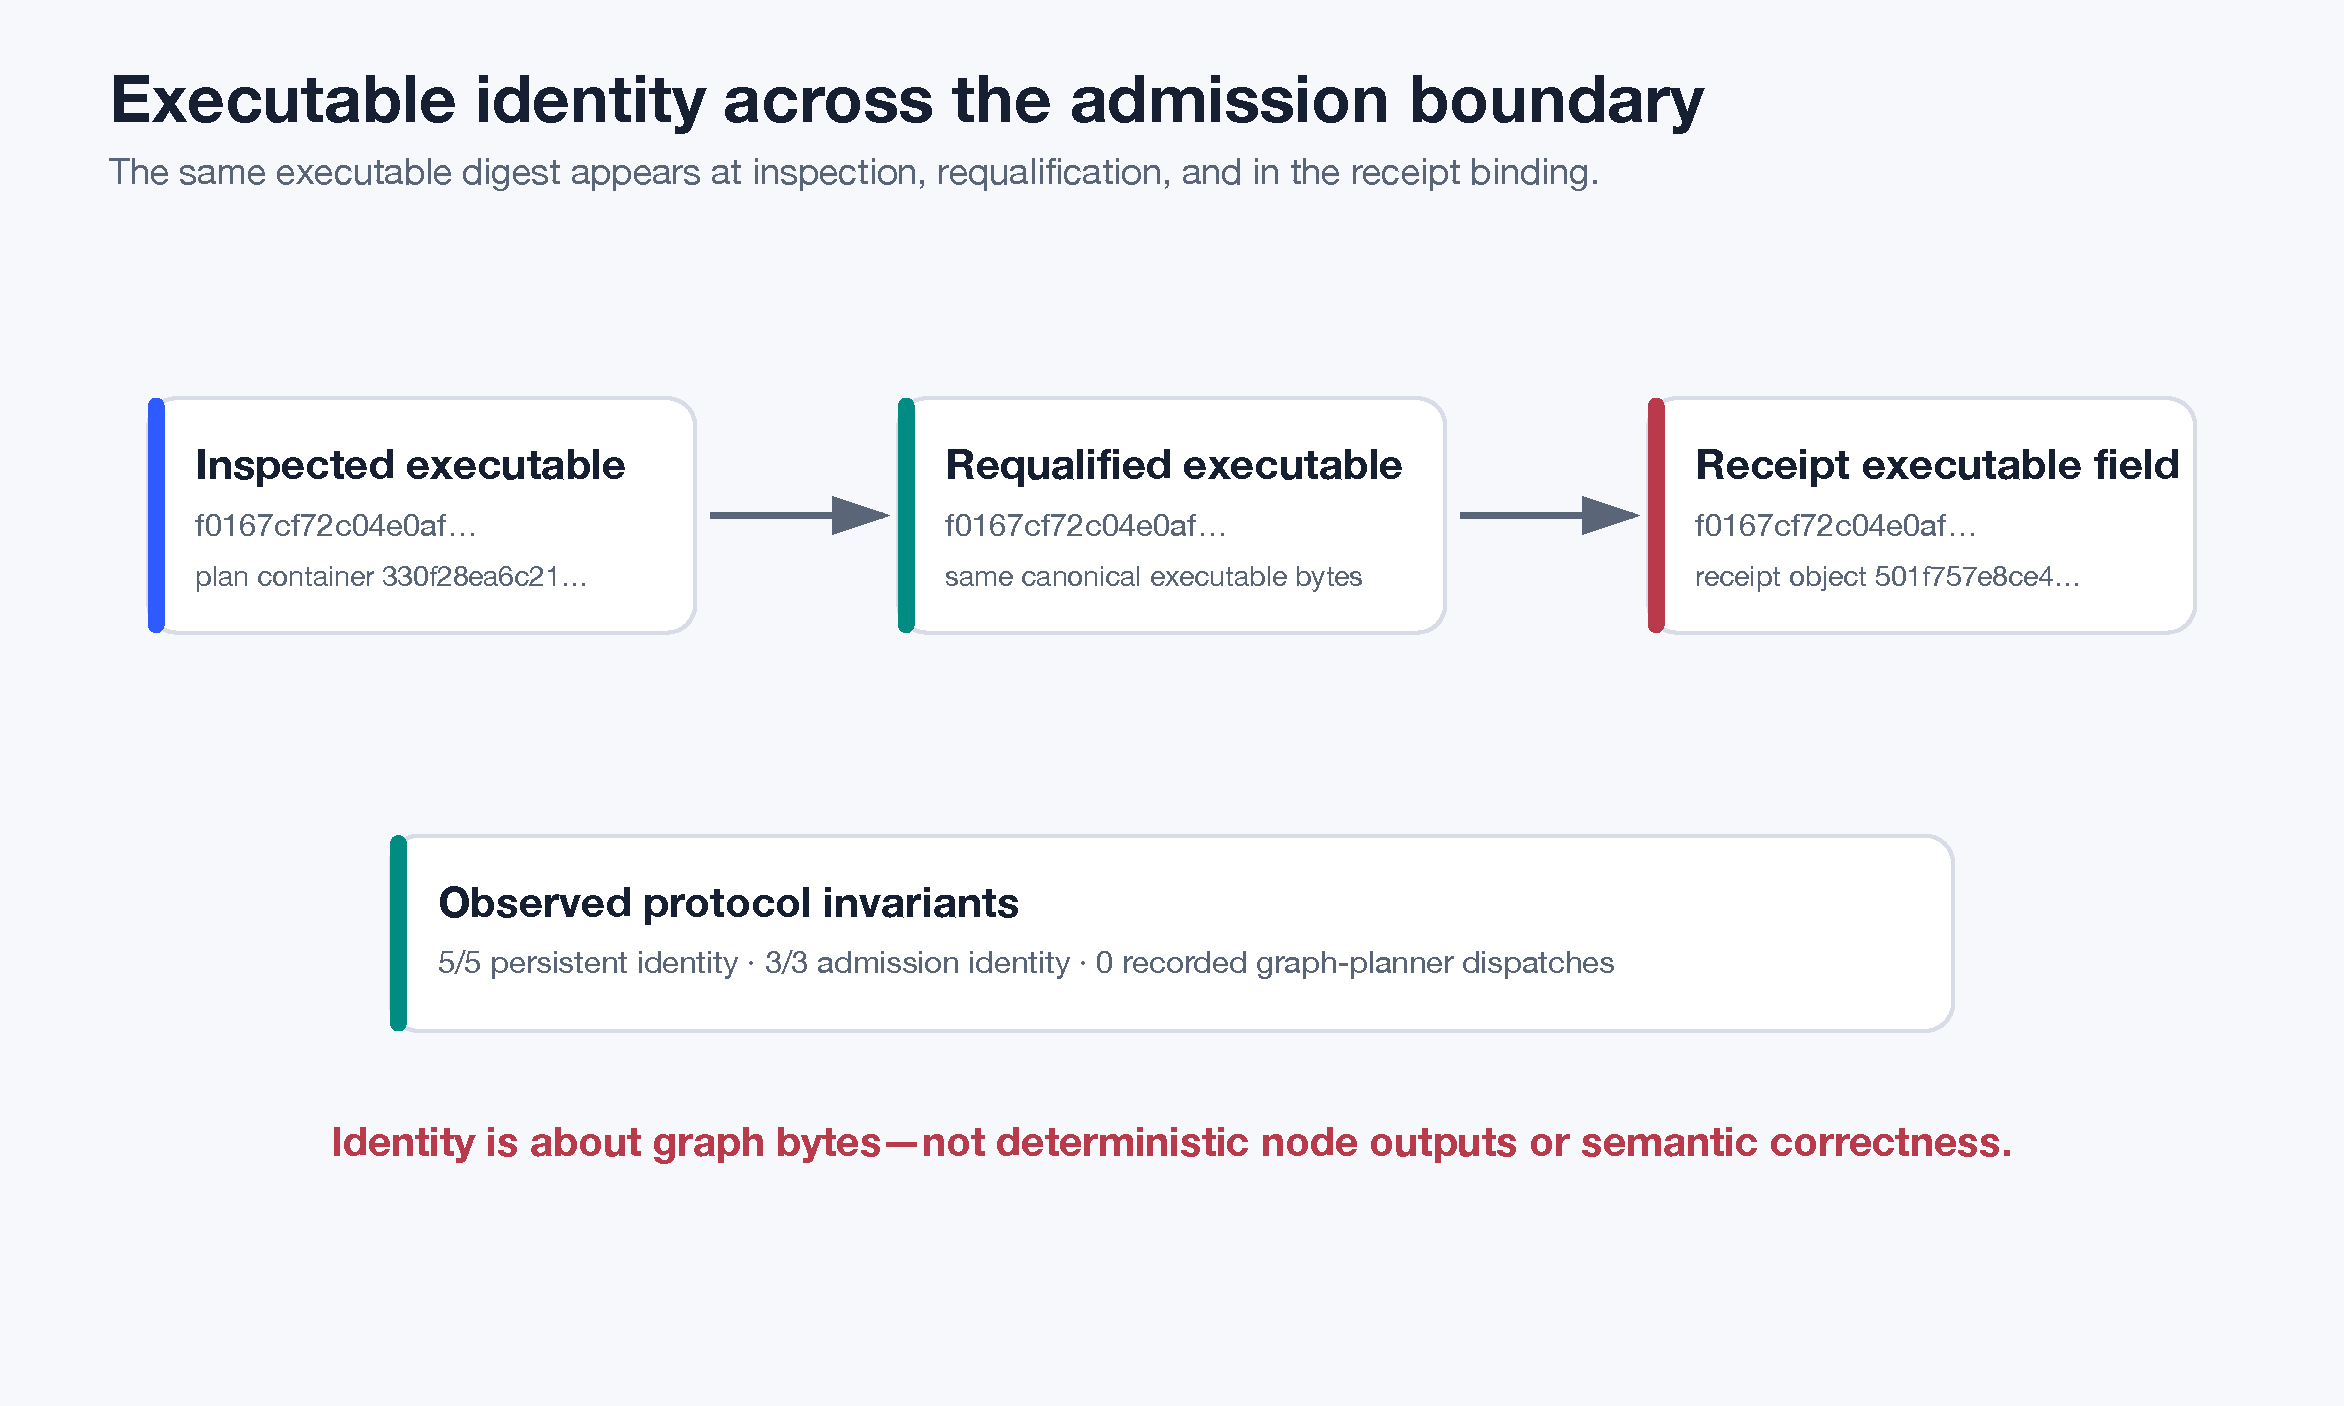
\includegraphics[width=0.92\linewidth]{figs/fig3-runtime-paths.pdf}%
  }{%
    \FigurePanel{Historical runtime identity chain}{%
      Inspected plan bytes $\rightarrow$ canonical executable hash
      $\rightarrow$ requalification $\rightarrow$ admission receipt binding
      $\rightarrow$ SequenceRunner.%
    }%
  }
  \captionof{figure}{One representative historical C30 identity chain at
  \code{\MentuCommitShort}. The \ExecutionCount{} admitted attempts carried
  distinct executable hashes. The receipt has its own identity while binding the
  requalified executable identity. This is pilot evidence, not a depiction of
  the later Core extraction.}
  \label{fig:runtime-paths}
\end{center}

The measurement pipeline has three layers. The frozen C30 analyzer remains the
authoritative interpretation of the pilot corpus.  Paper-local reproduction
independently recomputes the identity and manifest invariants, reports source
facts from committed blobs, and writes immutable JSON projections consumed by
the manuscript and figures.  It neither invokes the \mentu{} CLI nor writes to
the measured stores or sealed run bundles. Finally, disposable seeded controls
mutate copies only: one executable-bound contract field, one planner-lane
record, and one manifest-listed byte. A separate control independently executes
the committed current-Core admission-drift test in external build scratch.
These controls assess detector sensitivity in two separately reported epochs;
they are not
C30 observations, a reliability coefficient, or complete I5 coverage.

The unit of an identity check is an addressable artifact transition, not an
independent task trial.  Qualified plan stages may be counted for projection
parity; saved-plan execution attempts may be counted for inspection-to-receipt
identity.  They may not be treated as repeated outcome trials because the code
and plan evolved during debugging.  Human semantic inspection decisions are
retained as human judgments and are not recoded as mechanically derived
verdicts.

The pilot can falsify a protocol invariant: a receipt mismatch, an
execution-time planner dispatch, or a manifest mismatch would be a concrete
failure.  It cannot estimate a static-versus-dynamic-versus-hybrid effect
because the objective has no matched S or D arm.  It also cannot establish
planning amortization because there is no unchanged-state
\RegisteredRepeatCount{}-repeat series.

\section{Results and negative findings}

The mechanically regenerated pilot summary is shown in
Table~\ref{tab:pilot-results}. Its tabulated measurements and the principal
counts in the surrounding prose are injected from generated result artifacts
through the build context. Generated JSON remains authoritative where
explanatory prose restates a small corpus descriptor.

\begin{table}[htbp]
\centering
\small\rmfamily
\begin{tabularx}{\linewidth}{@{}P{0.34\linewidth}P{0.15\linewidth}P{0.13\linewidth}Y@{}}
\toprule
Check or observation & Type & Result & Context \\
\midrule
Persistent-projection executable identity &
Transition check & \PersistentIdentityCount/\QualifiedPlanCount &
Qualified plan projections \\
Recomputed admitted-bundle-to-receipt identity &
Transition check & \RecomputedAdmissionIdentityCount/\ExecutionCount &
Saved-plan executions \\
Graph-planner dispatches in saved-plan execution &
Event count & \ExecutionPlannerDispatches &
\ExecutionCount\ saved-plan executions \\
Sealed-manifest file-digest mismatches &
Leaf validation & \ManifestFileMismatchCount &
\ManifestFileCount\ file checks \\
Derived bundle-digest mismatches &
Aggregate validation & \ManifestBundleMismatchCount &
\ManifestBundleCount\ bundle checks derived from those file sets \\
Distinct discovery repository heads &
Corpus descriptor & \DistinctDiscoveryHeads &
\QualifiedPlanCount\ plan stages \\
Mechanically qualified plans rejected semantically &
Human judgment & \SemanticPlanRejections/\QualifiedPlanCount &
Plan inspection \\
Qualified projections selected for saved-plan execution &
Selection funnel & \ExecutionCount/\QualifiedPlanCount &
Versions v2 and v4 were not attempted after contemporaneous semantic rejection \\
Successful outputs requiring semantic correction &
Human judgment & \PostRunCorrectionCount/\ExecutionSuccessCount &
Completed outputs \\
Documented intervention decisions &
Chronology & \DocumentedInterventions & Full pilot history \\
Completed execution attempts &
Chronology & \ExecutionSuccessCount &
\ExecutionCount\ chronological attempts \\
\bottomrule
\end{tabularx}
\caption{Historical C30 invariant-exercise results. Every row derives from
\PilotObjectiveCount{} H-scaffold objective
(\(n=\PilotObjectiveCount\)) carried through sequential development stages;
the counts are not independent task trials.}
\label{tab:pilot-results}
\end{table}

The identity checks passed on the observed transitions:
\PersistentIdentityCount{} of \QualifiedPlanCount{} persistent projections and
\RecomputedAdmissionIdentityCount{} of \ExecutionCount{} independently
reconstructed requalified-bundle-to-receipt transitions retained executable
identity. Saved-plan execution recorded
\ExecutionPlannerDispatches{} graph-planner dispatches. The sealed-bundle audit
found all \ManifestFileCount{} expected leaves available, with zero missing and
zero extra. It found \ManifestFileMismatchCount{} mismatches across those
\ManifestFileCount{} file-digest checks and
\ManifestBundleMismatchCount{} mismatches across \ManifestBundleCount{}
aggregate checks derived from the same file sets. These
observations support identity continuity and planner separation in this corpus.
The transition funnel is explicit: five qualified projection attempts produced
five identity checks; contemporaneous human inspection rejected v2 and v4
semantically, so three projections were selected for saved-plan execution.
Those three execution attempts produced zero
requalification refusals, zero admission refusals, three admissions, and three
identity matches. The ratios are conditional transition checks, not end-to-end
pipeline success rates.
The planner result is additionally corroborated by
\PlannerClassifiedCallLaneRecordCount{} planner-classified and
\UnboundCallLaneRecordCount{} unbound records among the sealed execution call
lanes and by the pinned
saved-plan source path.  It does not imply that node-level model calls were
absent, and none of these observations implies deterministic node output.

The historical paper-local sensitivity exercise detected
\HistoricalDetectorControlPassCount{} of
\HistoricalDetectorControlCount{} named faults. A
mandatory contract-field mutation changed executable identity; an injected
planner-lane record changed the planner count from zero to one; and one byte
flip caused exactly \DetectorLeafFailureCount{} of \ManifestFileCount{} leaf
digests and \DetectorBundleFailureCount{} of \ManifestBundleCount{} derived
bundle digests to fail. Separately, the current-Core sensitivity exercise
detected \CurrentDetectorControlPassCount{} of
\CurrentDetectorControlCount{} named faults: its admission-drift test refused
a seeded captured-state mutation before execution. Input-tree fingerprints were
identical before and after. These are positive controls for the named
detectors, not additional pilot trials or proof of complete canonicalizer
coverage. The historical payload-mutation control exercises one of the six
mandatory \(F_\chi\) classes (\(\kappa\), contracts), with no historical
equivalence, \(F_\eta\)-isolation, header-mismatch, or omission-witness
fixture.

The \QualifiedPlanCount{} plan stages span
\DistinctDiscoveryHeads{} discovery repository heads, so the corpus is not
wholly fixed-state: v1 maps to \code{c0adef6}, v2 to \code{37f9f2c}, and
v3--v5 to \code{a828e91}. Thus the last three stages share a discovery head,
while their plans and executable identities still differ. The
\ExecutionCount{} saved-plan
executions are likewise chronological attempts, of which
\ExecutionSuccessCount{} completed the task.  Reporting that fraction as a
success rate would manufacture independence the design does not have.  The
\ExecutionCount{} admission receipts also bind \ExecutionCount{} distinct
executable hashes: no
executable graph was repeated, so the pilot contains no empirical comparison
of output reproducibility for an unchanged graph.

The \ManifestFileCount{} leaf checks are nested inside
\ManifestBundleCount{} bundles inside one pilot corpus. They are not
\ManifestFileCount{} independent trials, and no effective sample size of
\ManifestFileCount{} is claimed. The byte-flip control illustrates the
nesting: one changed leaf invalidated its leaf digest and the one derived
bundle digest that contained it.

The strongest negative result concerns semantic validity.
\SemanticPlanRejections{} mechanically qualified plans were rejected by human
semantic inspection, and \PostRunCorrectionCount{} mechanically successful
output required post-run semantic correction.  Mechanical qualification and
step verification therefore did not establish plan adequacy or outcome
correctness in the observed case. This is not an argument against
qualification; it identifies the boundary of what those predicates certified.

The attempt chronology documents \PlanningDispatchAttemptLowerBound{}
task-planning dispatches. Complete telemetry exists only for the
\QualifiedPlanCount{} saved qualified plans: \PlanningInputTokens{} input plus
\PlanningOutputTokens{} output tokens, totaling \PlanningTokenLowerBound{};
\PlanningElapsedMilliseconds{} milliseconds elapsed;
\PlanningRequestBytes{} request bytes; and \PlanningResponseBytes{} response
bytes. The other documented dispatches lack complete telemetry, so these exact
values are lower bounds for the full planning history rather than rounded
estimates or a treatment effect. The \ExecutionCount{} admitted
attempts contain incomplete USD-labelled model-cost telemetry. The
\KnownCostAttemptCount{} attempts with nonzero telemetry have a
US\$\ExecutionCostRoundedUSD{} subtotal; the remaining
\IndeterminateCostAttemptCount{} term is indeterminate because its recorded
zero cannot be distinguished from missing telemetry. The provider
pricing table used at collection time was not preserved, so no price
recalculation or completeness claim is made. The same history contains
\DocumentedInterventions{} documented intervention decisions across provider,
product, authority, plan, execution, and artifact-review stages.  With
\MatchedStaticCount{} matched S observations and \MatchedDynamicCount{} matched
D observations, none has a comparative interpretation.  The number of
unchanged-state repetition series is \UnchangedRepeatSeries.  The
machine-readable comparative-verdict flag is
\code{\ComparativeVerdictPermitted}, read from the repository artifact
\code{results/detector-sensitivity.json} (sha256 \code{18584045\ldots});
the artifact is named because it sits outside any blind-review surface
(finding BR9-007).

For the historical population, the evidence-adequacy vector is
\[
\Gamma_E=(\RecordedHostBoundaryRunCount,\,3,\,5,\,\ExecutionCount,\,0,\,
\varnothing,\,\varnothing,\,\omega_{0}):
\]
all three admitted runs have recorded host-boundary activity, three distinct
admitted executable identities, five projections, three invocations in the
reported I1 set, zero exercised header-refusal fixtures, zero exercised I4 drift
categories, zero C30 I5 fixture classes, and the published observation
profile \(\omega_{0}\) of Section~3. The first component is
instrumentation evidence, not proof that every semantic effect was captured.
Current-Core engineering tests and paper-local seeded controls are reported
outside this vector.

\clearpage
\begin{figure}[htbp]
  \centering
  \IfFileExists{figs/fig4-evidence-boundary.pdf}{%
    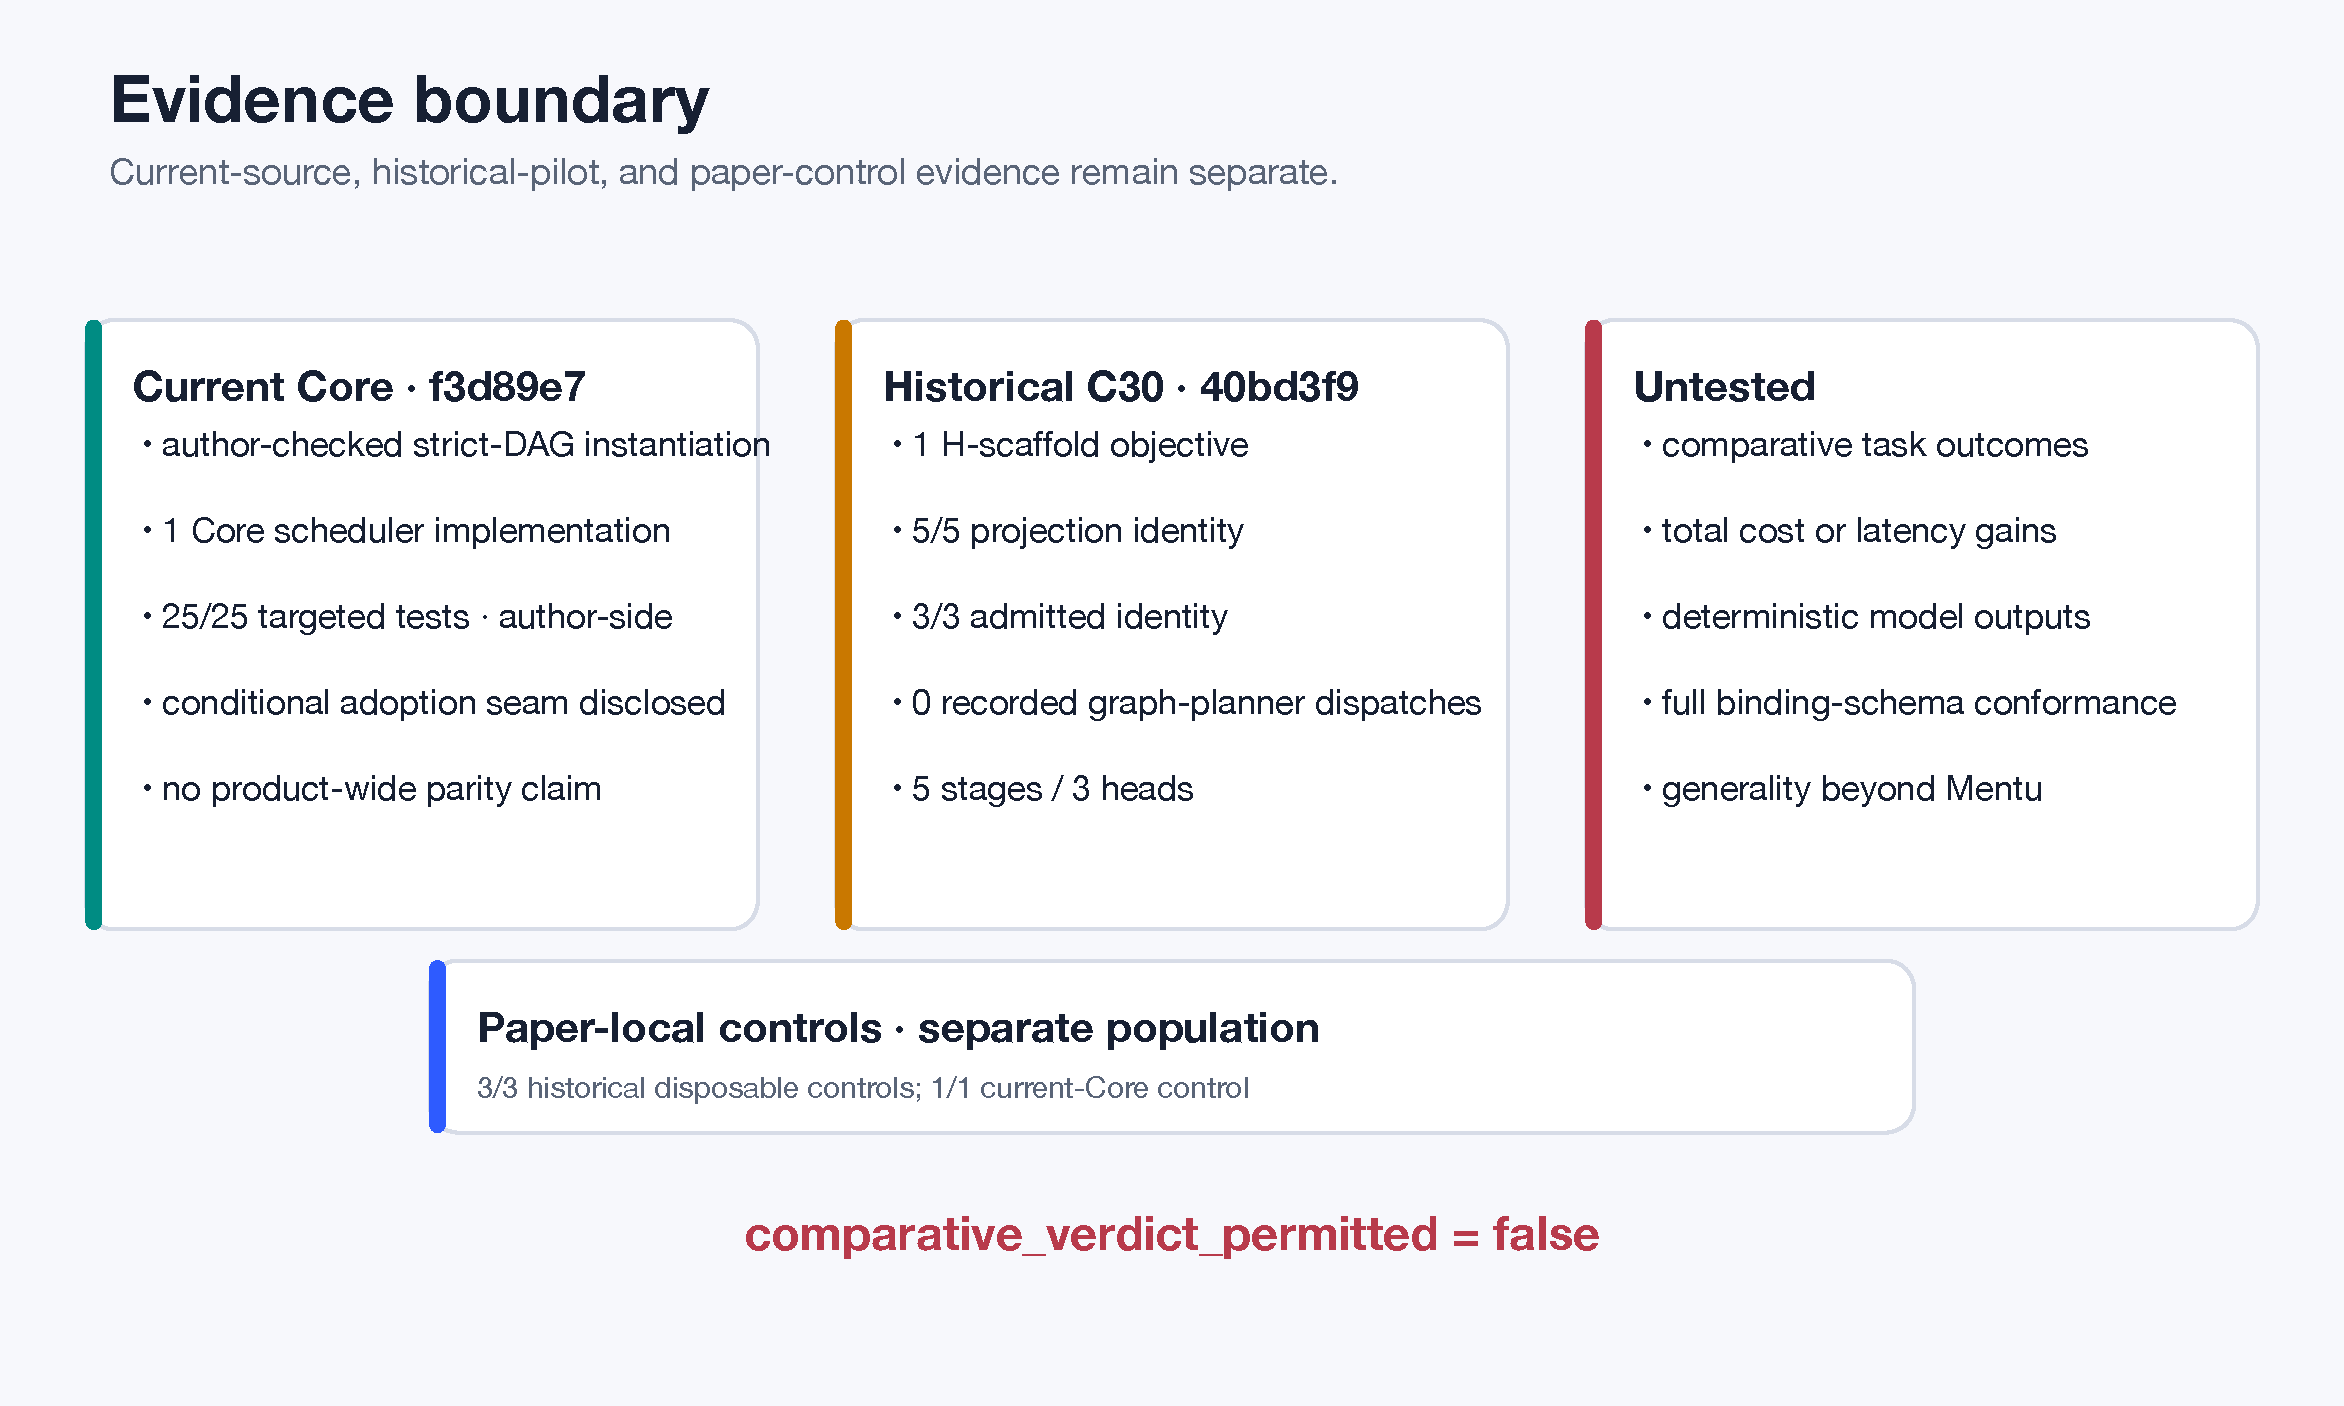
\includegraphics[width=\linewidth]{figs/fig4-evidence-boundary.pdf}%
  }{%
    \FigurePanel{Evidence boundary}{%
      Supported: the author-checked strict-DAG Core instantiation at the current pin;
      observed: staged identity and planner separation in the historical pilot;
      untested: comparative outcomes, amortization, semantic superiority,
      cross-platform generality, and literature novelty.%
    }%
  }
  \caption{Claim boundary for \PaperVersion.  Observed protocol properties do
not license unmeasured treatment effects.}
  \label{fig:evidence-boundary}
\end{figure}

\section{Discussion: Object Graphs, Lifecycle Control, and Successor Epochs}

The model admits a layered architectural reading.  The executable task graph is
the object-level course of action: it fixes effect-bearing nodes, contracts, and
scheduling relations.  The lifecycle state machine is a meta-level control
structure: it records how that object was proposed, which predicates were
established, when its identity became addressable, which concrete context
authorized effects, and what evidence survived execution.  ``Meta-level'' is
used in an engineering sense; it does not ascribe self-awareness, privileged
introspection, or semantic understanding to the runtime.

The separation changes the meaning of agent governance.  \mentu{} does not make
stochastic agent behavior deterministic.  It makes an executable commitment
inspectable and its authority to act attributable.  Construction may remain
exploratory before admission.  Once an exact graph epoch has gained effect
authority, however, a change to effect-bearing topology or scheduling semantics
requires either a separately admitted successor epoch or an admitted outer
transition system whose identity includes the planner and permitted transition
relation.  Dynamic construction and governed execution are therefore
compatible without collapsing proposal into authority.

Execution evidence is not by itself a graph-update operator, and preservation
is not learning.  A cross-epoch extension could allow evidence and review to
inform construction of a successor graph, but that successor would still
require lowering, qualification, and admission.  This represents recursive
adaptation as an authorized lineage of graph epochs rather than silent mutation
of an already admitted graph.  The present paper establishes the within-epoch
substrate and the boundaries such an extension would have to preserve; it does
not claim that cross-epoch learning is implemented or beneficial.

\section{Threats, boundaries, and limitations}

\paragraph{Construct validity.}
The model makes graph identity narrower than result reproducibility and
both plan adequacy and outcome correctness. The versioned binding schema makes
topology, node behavior, contracts, graph-declared scheduling, policy, and
toolchain identity-bearing: effect-semantic fields enter \(F_\chi\), while the
exact toolchain and schema header enters \(F_\nu\) before payload
canonicalization. Declared closure, payload equivalence/inequivalence,
partition isolation, header matching, and omission probes are separate tests.
This improves falsifiability but does not prove that the chosen schema captures
every causally relevant fact. A model selector frozen by the executable is
mandatory in executable identity; an independently resolved route,
scheduler-build identity, provider runtime state, and authority state belong in
the declared residual environment binding. The pilot binds declared
environment constituents through qualification and admission records but does
not compute one aggregate environment digest, so it cannot report
\(h_{\eta,1}=h_{\eta,2}\).  A collision-resistant digest is evidence about
identical encoded objects, not about the adequacy of the encoding.

\paragraph{Internal validity.}
The C30 corpus records a development pilot whose implementation, authority
configuration, and plans changed between stages.  Its \DistinctDiscoveryHeads{}
repository heads make that evolution visible, but they also prevent a
fixed-state outcome interpretation.  Human semantic rejections and the
post-run correction are important negative evidence, yet they were made by
the author-operator during development rather than by blinded raters. Some
telemetry, including human inspection time and a complete execution-token
account, was not available.  The pilot challenged zero drift classes; drift
refusal remains prospectively specified but empirically untested in C30. The
seeded current-Core drift control is separately labeled engineering-test
evidence and does not change that denominator.

\paragraph{External validity.}
The empirical material is confined to the observed H-scaffold objective. The
current implementation mapping is confined to \mentu{} as the author-checked
architectural instantiation. Its admitted profile accepts strict DAGs, whereas the
abstract model allows a wider graph class. The mapping therefore demonstrates
one coherent realization, not cross-platform generality or comparative rank.
Systems with runtime topology mutation, open-ended tool arbitration, or
different authority models may need multiple admitted epochs or a different
abstraction.

\paragraph{Comparative boundary.}
There are no matched S or D observations, no H-direct control, and no
unchanged-state repetition series.  The paper cannot infer lower total cost,
lower latency, fewer regressions, reduced intervention, improved task success,
or planning amortization.  Static authoring effort and human inspection effort
would need explicit measurement in any such comparison.

\paragraph{Implementation boundary.}
The current admitted profile has a closed Core definition, qualification and
admission primitives, activation evidence, and one Core scheduler. General
recipes and interpreted workflows remain compatibility profiles with
different authority or runner contracts. The source audit does not enumerate
every non-graph effectful product operation, so it makes no product-wide
coverage percentage. It also finds that persistent generated projections can
re-enter legacy recipe dispatch without explicit adoption. That cross-profile
transition is a real adoption boundary; it neither erases the admitted Core
nor licenses a claim of uniform admission.

\paragraph{Scholarly and review boundary.}
\ifdefined\InternalBuild
A bounded set of cited primary records from earlier cycles has had its source
identity independently reconciled and its claim-specific use explicitly
dispositioned. The v0.9.5 exact-input return passed its mechanical isolation
gate, but independent audit found five copy-contaminated RFC author fields, a
34-of-37 honest citation-entity crosswalk, and one mutable-versus-pinned source
drift. Its literature coding is bounded discovery evidence and its blind
review is major-revision input, not certification. This revision therefore
also records that v0.9.6 failed its full raw gate and v0.9.7 failed independent
trace audit despite a green structural validator. The latter return's 43/43
cite-key identity crosswalk does not certify full rendered bibliography
metadata, and its RFC~2748 record fails the protocol's first-author condition.
This revision therefore requires a fresh exact-input, trace-audited run; no
priority, exhaustive-coverage, or novelty claim is licensed.
\else
  \ifdefined\VerifiedLiterature
    The cited primary records were checked against an input-bounded literature
    registry, and an exact-input blind review of the internal PDF and public
    supplement was separately dispositioned. Their represented process events
    were checked against two supplied closed-session exports. These controls
    reduce positioning and review error within their declared protocols; they
    do not prove export or search completeness, universal novelty, priority, or
    cross-platform generality.
  \else
    \PackageError{agent-graph-runtime}{Missing publication mode}{%
      Build with build.py in internal or release mode.%
    }%
  \fi
\fi

\paragraph{Privacy and reproducibility boundary.}
The public package uses digests, summaries, committed blob identities with
path-and-line locators, and
path-neutral scripts.  It excludes credentials, transcripts, raw session
exports, private filesystem paths, and sealed run-bundle contents.  This
protects private material but means that some sealed evidence must be verified
by an authorized local reproducer rather than redistributed. Bare hashes of
short source lines are deliberately excluded because they are guessable and
provide no confidentiality. Timestamp-suffixed run identifiers and the pilot's
single-operator telemetry may support work-pattern inference. They are
explicitly not privacy controls. The current artifact remains internal. A
public release must either publish a pseudonymized projection whose invariants
still pass or record the author-operator's explicit consent to the retained
activity data. Before a future study records other humans' authoring or
inspection time, its protocol must document an ethics determination and a
consent procedure; the present pilot is single-operator and supplies neither
for a multi-participant study.

\section{Prospectively committed matched-study protocol}

The adjudicating study was specified in the author-controlled C30 record before
the pilot evidence and is restated here to separate future inference from
pilot interpretation. No external registration timestamp is claimed. It
freezes at least
\RegisteredObjectiveMinimum{} objectives spanning at least
\RegisteredTaskFamilyMinimum{} task families and
\RegisteredSizeStrataMinimum{} size strata.  Each objective is executed in S,
D, H-scaffold, and H-direct arms on resettable repository fixtures. The floor
of \RegisteredObjectiveMinimum{} objectives is an instrument-operability
threshold, not a power justification. Before inferential execution, a
precision analysis will set the final corpus size from the target width of the
paired verified-completion interval. Backend,
execution model, authority envelope, token and cost ceilings, and mechanical
verification contracts are held constant within objective.

Arm order is randomized within objective, and every attempt is retained,
including pre-dispatch refusals and execution failures.  Static recipes are
authored before randomized execution begins; their human or model authoring
time is measured rather than treated as zero.  H-scaffold and H-direct share
the staged freeze policy so their contrast isolates authoring method more
cleanly than a comparison with D.  S and D provide the persistent and
continuous-invocation reference policies.

The primary comparative endpoint is verified task completion. Exact executable
identity, planner-dispatch count by lane, pre-effect drift refusal, and
manifest integrity are protocol-conformance outcomes. Secondary comparative
endpoints are intervention count, elapsed time, model cost, planning tokens,
authoring time, inspection time, and typed refusal rate. A hierarchical
analysis tests the primary endpoint first; secondary intervals use a Holm
family-wise adjustment and unadjusted estimates are labeled exploratory.
Every eligible first attempt---including a refusal or failed
execution---enters the primary analysis and is followed by
\RegisteredRepeatCount{} unchanged-state invocations when the arm remains
operationally eligible. Reuse and amortization are reported both
unconditionally and, separately labeled, conditional on an admitted first
execution. Outputs may vary; the executable identity requirement does not.

Analysis is paired by objective.  It reports arm-specific distributions,
paired differences, medians, and bootstrap confidence intervals rather than
promoting pilot counts to population estimates.  Refusals are safety outcomes,
not silently recoded task successes or failures.  Deviations, exclusions, and
missing telemetry remain visible.  The detailed execution and adjudication
rules appear in the appendix.

\section{Conclusion}

Static, dynamic, and staged-hybrid agent execution need not imply separate
runtimes.  They can be represented as policies over when a graph is
constructed, where it freezes, how it is authored, and which substrate executes
the admitted result.  That abstraction is useful only if it preserves the
boundaries among executable identity, environment identity, output
reproducibility, plan adequacy, outcome correctness, and authority.

\mentu{} operationalizes the model's central separation through an extracted
Core with a public API that owns the closed executable, qualification and
admission primitives, activation evidence, and strict-DAG scheduler. Engine
adapters supply host effects, while named compatibility profiles retain
different contracts. The audit also exposes the next coherent hardening step:
persistent generated projections need an explicit adoption transition before
they can enter a different assurance contract.

The historical C30 checks passed on their observed identity and planner-lane
transitions, while preserving semantic failures that mechanical qualification
did not catch. Seeded controls show sensitivity to
\HistoricalDetectorControlPassCount{} of
\HistoricalDetectorControlCount{} named historical faults; a separate
current-Core control detected \CurrentDetectorControlPassCount{} of
\CurrentDetectorControlCount{} current fault. Neither result supplies a
comparative verdict, aggregate environment-identity result,
unchanged-graph output repeat, or complete I5 conformance claim.

The next scientific steps are therefore bounded: literature-check and
blind-review exactly this frozen internal PDF and supplement in isolated
contexts, then run the prospectively committed matched study. Until those gates
close, the contribution is a testable lifecycle model, an author-checked
architectural instantiation, an implementation-boundary finding, and a bounded
invariant exercise---not a claim of novelty, universality, comparative rank,
status, or superiority.

\appendix
\section*{Appendix: Evidence, claims, and matched-study detail}
\addcontentsline{toc}{section}{Appendix: Evidence, claims, and matched-study detail}

\subsection*{A. Provenance and evidence grades}

Table~\ref{tab:provenance} names the manuscript's load-bearing source classes.
Repository-local paths are resolved by the reproduction wrapper; no private
absolute path is part of the paper source or public package. Input digests and
the complete file-level mapping are recorded in \code{SOURCE-MAP.md} and the
generated evidence manifest.

\begin{table}[htbp]
\centering
\small
\begin{tabularx}{\linewidth}{@{}P{0.19\linewidth}P{0.24\linewidth}Y@{}}
\toprule
Source & Pinned identity & Permitted use \\
\midrule
C30 prospective protocol & \code{\CThirtyPreregCommitShort} & Frozen definitions,
predictions, falsification rules, and matched-study design \\
C30 pilot corpus & \code{\EpistemicsEvidenceCommitShort} & Read-only
historical invariant-exercise observations and negative findings \\
\mentu{} historical source & \code{\MentuCommitShort} & C30-era source
corroboration only \\
\mentu{} current source & \code{\MentuCurrentCommitShort} & Current Core,
adapter, scheduler, admission, compatibility-profile, and projection-adoption
facts \\
Structural Waste & \code{\StructuralWasteCommitShort} & Methodological
discipline only; no substantive theory transfer \\
Claude Science exports & External raw inputs, excluded from Git & Provenance of
failed attempts and bounded Operon returns; raw session
frames are not release evidence \\
\bottomrule
\end{tabularx}
\caption{Source roles. Committed source and frozen reproducible analysis are
internally high-assurance author-produced evidence; sealed hash-checkable local
artifacts are access-restricted; dirty worktree and vendor-reported
observations are non-load-bearing. These grades do not claim independent
public replication.}
\label{tab:provenance}
\end{table}

The external research exports are retained outside the repository.  The first
export referenced \path{ground_truth.json}, which was unavailable; no
reconstruction is treated as equivalent.  The earlier 29 July return exported
an older manuscript-construction task and never received the target PDF or
public supplement. The first 30 July return matched the task but failed the
isolation and exact-input contract; its canonical artifacts remain preserved
as advisory evidence. The subsequent v0.9.3 rerun passed the reported
memory-isolation and exact-two-file input gate and is preserved byte-for-byte
under \code{operon-v093/}. Its green attestation records the declared process
conditions, not substantive correctness; the blind review recommended major
revision. The later exact-input v0.9.4 return is preserved byte-for-byte under
\code{operon-v094/}; independent audit overrides its coordinator's green
narrative because the frozen raw-return validator fails. Downloaded source maps
were replaced by a repository-owned corrected map rather than overwritten.
The v0.9.5 return is preserved under \code{operon-v095/}. Its isolation gate
passes, while independent audit rejects literature certification because five
RFC author records are copy-contaminated and the citation registry cannot be
honestly crosswalked one-to-one to all cited entities. Its 44-finding blind
review remains major-revision evidence.
The v0.9.6 return is preserved as a failed raw-gate epoch with 21 advisory
findings, six major. The v0.9.7 raw files are also preserved byte-for-byte, but
their green structural result is overridden for release purposes by the private
session trace: Contexts A and B overlapped, both read undeclared text
derivatives, automated reviewers crossed the claimed boundary, and the same
Context A was resumed to repair a failed full-validator result. Its 21 findings
remain advisory repair inputs; the run supplies no release authorization.
Uncommitted terminal and GUI evidence is recorded only as internal provenance.

The v0.9.9 certification program ran six sealed protocol epochs (r1--r6),
and every one ended honestly without producing a certifiable review. r1 and
r2 stopped in preflight on frozen vocabularies that lacked a term for
something the platform emitted. r3 reached adjudication and returned
noncompliant on six codes. r4 stopped on a contradiction between two pinned
protocol documents; r5 on a supplied export of a session that had never
finished. r6 — with custody preflights closing every previously discovered
gap — reached adjudication and returned noncompliant on seven
producer-conduct codes, principally the divergence of producer
self-describing logs from the platform-represented trace: fifty-seven logged
network requests against zero represented network events, and one hundred
four file-open claims contradicted by the represented event scan. Each
epoch's raw tree, toolchain, and stop or void record is preserved
byte-for-byte under its own lineage
(\code{provenance/OPERON-V099*\allowbreak.md},
\code{operon-v099*/}, \code{operon-certification-v099*/}). The r6 blind
reviewer satisfied its own distinguishing constraints, and its seven findings
are dispositioned in the supplement as uncertified advisory review; findings
BR9-001 through BR9-007 are addressed or scheduled in this candidate. By
dated author decision
(\code{provenance/RELEASE-BOUNDARY-DECISION-2026-08-14.md}), a certified
review is no longer a release precondition; disclosure of this six-epoch
record is. The repeated adjudication result — that unverified producer
self-reports diverge from platform-represented traces — is itself evidence
for the position this paper takes on trace-derived, rather than
self-attested, process records.

\subsection*{B. Manuscript-facing claims ledger}

This manuscript and its co-reviewed reproducibility supplement are
authoritative for public-facing claims. The machine-readable
\code{spec-map.json} and full \code{CLAIMS-LEDGER.md} are internal audit
metadata and must not broaden this reviewed surface. Table~\ref{tab:claims}
is the complete manuscript-facing projection of the material claim classes.

\begin{table}[htbp]
\centering
\small\rmfamily
\begin{tabularx}{\linewidth}{@{}P{0.13\linewidth}P{0.18\linewidth}YP{0.16\linewidth}@{}}
\toprule
ID & Class & Claim & Status \\
\midrule
\code{AGR-AD-01} & architectural definition & Construction time, freeze
boundary, authoring method, and execution substrate are separately specified
coordinates over a constrained feasible region. &
Defined here; precedents positioned without novelty claim \\
\code{AGR-FP-05} & formal implication & Multiple policy configurations can target one
executable IR and substrate without sharing an authoring path. & Conditional on
the model \\
\code{AGR-IF-11}\newline\code{AGR-IF-12} & implementation fact &
\code{MentuExecutionGraphCore} owns the admitted definition, lifecycle,
qualification, admission, activation evidence, and DAG scheduler; engine
adapters supply effects. & Current-head source plus 25/25 targeted author-side
tests; no product-wide cross-origin execution claim \\
\code{AGR-IF-13} & implementation fact & Persistent generated projection can
re-enter ordinary recipe discovery without an explicit adoption transition. &
Current cross-profile transition boundary \\
\code{AGR-IF-14} & implementation fact & \mentu{} is the author-checked
architectural instantiation of the strict-DAG admitted profile. &
Profile-scoped synthesis; not
a comparative rank \\
\code{AGR-PO-01}\newline\code{AGR-PO-02} & pilot observation & Saved-plan and persistent-projection
identity held on all observed artifact transitions. & Noncomparative pilot
evidence \\
\code{AGR-PO-03} & pilot observation & Saved-plan execution contained no
recorded graph-planner dispatch in the observed attempts. & Noncomparative pilot
evidence \\
\code{AGR-PO-06}\newline\code{AGR-PO-07} & pilot observation & Mechanical qualification did not
establish plan adequacy or outcome correctness in the observed case. &
Negative result retained \\
\code{AGR-EX-01} & excluded claim & Staging improves success, total cost,
latency, intervention, maintenance, or regression outcomes. & Not permitted \\
\code{AGR-AD-06} & architectural definition & Unadmitted runtime topology or
scheduling mutation is not another policy over one frozen graph epoch. &
Scope boundary retained \\
\bottomrule
\end{tabularx}
\caption{Claim classes and current dispositions. ``Supported'' is scoped to
the named evidence; it is not a cross-platform generality claim.}
\label{tab:claims}
\end{table}

\subsection*{C. Implementation and assurance-contract map}

Table~\ref{tab:convergence} separates shared execution machinery from
policy-specific assurance and topology contracts.

\begin{center}
\centering
\small\rmfamily
\begin{tabularx}{\linewidth}{@{}P{0.17\linewidth}YYY@{}}
\toprule
Layer & Admitted graph profile & Recipe compatibility profile & Interpreted
workflow profile \\
\midrule
Executable form & Core \code{ExecutionGraph\allowbreak Definition} through checked engine
adapter & General \code{SequenceDefinition} & Validated JavaScript program \\
Authority entry & Core qualification and admission before sole admitted runner &
Raw compatibility initializer with legacy authority & Separate
\code{WorkflowRunner} contract \\
Scheduling & One Core \code{ExecutionGraph\allowbreak Scheduler} for the admitted DAG &
DAG-shaped recipes may use the Core scheduler through the engine adapter;
raw compatibility routes use their selected \code{SequenceRunner} contract,
without a paper-wide scheduling-convergence claim & Interpreter-defined transitions \\
Evidence & Qualification, receipt, activation, call-lane, and run evidence &
Sequence/run evidence under the selected recipe contract & Workflow journal
and budgets; no admitted-meta-runtime claim here \\
Cross-profile transition & Projection stays in-profile or is explicitly
adopted & Generated projection can currently be rediscovered here without
explicit adoption & Not classified as a frozen inner-graph policy \\
\bottomrule
\end{tabularx}
\captionof{table}{\mentu{} runtime surfaces and assurance contracts at commit
\code{\MentuCurrentCommitShort}. The admitted Core is the named
instantiation; compatibility profiles are named rather than treated as missing
pieces of that Core.}
\label{tab:convergence}
\end{center}

\subsection*{D. C30 pilot interpretation rules}

The paper-local reproduction applies the following rules without rewriting the
frozen C30 result:

\begin{enumerate}
  \item Independently load each persistent recipe and prompt set, reconstruct
  its normalized definition, contracts, effective policy, and canonical
  executable digest, then cross-check the stored parity record.
  \item Compare the inspected executable identity with the requalified
  admission bundle and receipt for every admitted saved-plan execution.
  \item Count graph-planner dispatches only in the saved-plan execution
  invocation; admitted node-model calls belong to a separate execution lane.
  \item Recompute every available sealed-manifest entry and count mismatches
  without copying private contents.
  \item Count distinct discovery repository heads across plan stages to
  distinguish evolving debugging stages from unchanged-state repeats.
  \item Preserve human semantic rejection and correction records as human
  judgments; do not transform them into mechanical analyzer outputs.
  \item Set the comparative verdict to false whenever matched S and D arms or
  the registered repetition series are absent.
\end{enumerate}

An identity pass supports only the relevant artifact transition. A
pre-dispatch refusal is a safety outcome. A completed step is not semantic
certification. Sequential attempts are not independent trials. These rules
are enforced in the claims ledger as well as in prose.

\subsection*{E. Prospectively committed matched-study execution}

\paragraph{Experimental unit and corpus.}
The experimental unit is one frozen objective evaluated under all four policy
arms. The corpus contains at least \RegisteredObjectiveMinimum{} objectives
across at least \RegisteredTaskFamilyMinimum{} task families and
\RegisteredSizeStrataMinimum{} size strata. Objectives, eligibility rules,
task-family labels, size labels, fixture-reset procedures, and verification
contracts are frozen before the first randomized arm is executed.

\paragraph{Arms.}
\begin{description}
  \item[S:] a persistent recipe and prompts exist before the experimental task
  invocation; graph-planner dispatch during execution is zero.
  \item[D:] one task-time planner dispatch constructs, qualifies, and executes
  the graph continuously without an operator-visible frozen plan.
  \item[H-scaffold:] a scaffold-method task-time planner creates an
  addressable plan; a later invocation requalifies and executes those exact
  bytes.
  \item[H-direct:] the same staged boundary as H-scaffold with the direct
  authoring method, isolating staging from authoring style.
\end{description}

\paragraph{Controls and randomization.}
Each objective begins from a resettable repository fixture. Execution backend
and model, authority limits, token and cost ceilings, sandbox and permission
posture, expected-change scope, and mechanical verification remain matched.
Arm order is randomized within objective. Static artifacts are authored and
frozen before randomized execution; authoring labor and model usage are
recorded. Every invocation receives a stable objective identifier, arm,
order position, fixture identity, repository identity, authority-envelope
identity, and artifact lineage.

\paragraph{Attempt accounting.}
All attempts remain in the record. Eligibility requires valid authority,
available credentials and provider, no disqualifying fixture drift, and arrival
at qualification. Infrastructure refusals remain visible but are excluded
from task-success denominators according to the frozen rule. Human edits,
retry decisions, authority changes, and plan regenerations are interventions.
Mechanical drift refusals are typed separately. The analysis reports both the
intention-to-run history and the eligible-attempt subset.

\paragraph{Measurements.}
Protocol measures include planner dispatch count and lane, request and response
bytes, input and output tokens, elapsed planning time, candidate source
identity, executable identity, qualification identity, receipt identity,
manifest integrity, and pre-effect drift behavior. Operational measures
include verified completion, changed paths, execution duration, model cost,
interventions, typed refusals, and reusable artifacts. Human authoring and
inspection duration are timed explicitly. CLI-return latency is separated
from runner duration so post-run extraction cannot be mistaken for execution
latency.

\paragraph{Repetition and outcomes.}
After a successful first execution, each arm receives
\RegisteredRepeatCount{} unchanged-state repetitions from an equivalent reset
fixture. Graph identity is expected to remain exact where the policy freezes
an addressable artifact; model outputs are allowed to vary. The primary
falsification outcomes are any staged receipt identity mismatch, any
graph-planner dispatch during saved-plan execution, or any detected drift that
reaches effectful execution. Comparative outcomes remain descriptive until
the complete matched design is analyzed.

\paragraph{Analysis and reporting.}
Results are paired by objective. The report provides arm-level distributions,
paired differences, medians, bootstrap confidence intervals, missingness, and
typed refusal counts. H-scaffold versus H-direct estimates an authoring-profile
contrast under a shared staging policy; comparisons involving D or S change
additional lifecycle dimensions and are interpreted accordingly. No outcome
is promoted from the pilot. Deviations from the frozen protocol receive dated
amendments, and null or adverse findings remain in the release artifact.

\ifdefined\InternalBuild
  \subsection*{F. Operon release gate}

  The internal manuscript becomes eligible for a public preprint only after:

  \begin{enumerate}
    \item input-bounded discovery, followed by full-text or identifier checks,
    across agent frameworks, planner--executor systems, graph runtimes,
    planning, content-addressed builds, durable execution, provenance, and
    admission, in a separately closed review-domain session;
    \item a verified prior-art registry and literature matrix;
    \item blind review of exactly the internal PDF and public supplement in a
    second separately closed review-domain session, with a digest-bound
    deterministic text projection of that same PDF permitted only as a
    navigation aid, and with no network, Context A artifact, internal claims
    ledger, or spec map as input;
    \item detached derivation over both closed-session exports, scanning each
    root frame and its complete descendant closure for undeclared inputs,
    cross-domain references, and prohibited effects;
    \item explicit disposition of novelty, terminology, formal-soundness,
    empirical-overclaim, citation, and reproducibility findings; and
    \item an integrity build in which cited and bibliography sets match and no
    unverified identifier remains;
    \item author-owned publication clearance binding a public licence, a stable
    release locator, and explicit consent for retained timestamp-bearing
    activity data.
  \end{enumerate}

  \emph{Dated status.} The eligibility rule above records the gate as
  designed. By the author's boundary decision of 2026-08-14,
  certification ceased to be a release precondition (disclosure of the
  epoch record, incorporation of the uncertified blind-review
  dispositions, and the explicit release act are); the release act
  occurred on 2026-08-22 under Decision A1, with the machine gate's
  refusal of this candidate preserved undisturbed in the repository
  record rather than amended away.

  The machine gate treats the return as a closed evidence layout. It binds
  canonical prompt and preflight bytes, proves the declared text projection
  against the authoritative PDF, rejects undeclared local reads and all
  blind-domain network access, recomputes manuscript citation locations, and
  requires auditable receipts for source resolution and finding disposition.
  A review domain is the complete frame graph reachable from one exported root,
  not only its initiating frame. Declared reviewer or critic descendants inside
  that closure are therefore visible parts of the review computation; an edge,
  read, identifier, or artifact crossing from the literature domain into the
  blind domain is disqualifying. After both producers terminate, a separate
  Codex-side extractor reads and hashes the actual exports and derives the
  lifecycle, tool, artifact, and information-flow record. The producer cannot
  submit a substitute audit JSON or run the certifying validator. The raw
  exports remain private and outside the public package; the derived audit
  records only path-neutral identities, counts, locators, digests, and a scoped
  result.

  The result is explicitly relative to events represented in the supplied
  exports. Because those exports are not platform-signed completeness proofs,
  unobservable host controls remain unknown: an absence in the export is not
  promoted into proof that omitted platform state could not exist. Review
  independence, observable non-interference, artifact consistency, scholarly
  correctness, and author release authority are separate decisions.
  Release validation, the reviewed internal rebuild, and public packaging run
  from one frozen source snapshot. These controls establish byte identity,
  provenance, and review traceability; they do not mechanically prove
  scholarly correctness or semantic support.
  Search breadth and literature-matrix coding likewise remain attested
  scholarly process: the gate binds the returned artifacts but cannot infer
  exhaustive coverage or semantic correctness from their presence.

  Operon findings are review inputs, not automatic authority. The v0.9.5
  exact-input return supplied a substantive major-revision review and passed
  its frozen process gate, but its copy-contaminated and non-bijective
  literature registry cannot authorize release. The v0.9.6 return failed its
  raw gate. The v0.9.7 return demonstrates why self-attested isolation is also
  insufficient: its raw validator is green while trace audit is red. The
  v0.9.8 preflight adds the converse lesson: an unverifiable audit must stop
  before review rather than be completed by assertion. This revision changes
  the PDF, supplement, review protocol, and build projection. Each citation and
  revision remains subject to repository-owned verification and disposition.
  The r6 epoch then reached adjudication and returned noncompliant on seven
  producer-conduct codes; the six-epoch record is disclosed in Appendix~A.
  By the dated author decision of 2026-08-14, release no longer waits on a
  certified review; it requires the disclosed record, the incorporated r6
  uncertified-review dispositions, and the author's explicit release act.
\else
  \ifdefined\VerifiedLiterature
    \subsection*{F. Review certification boundary}

    The release record binds an input-bounded literature registry, its
    separately verified identifiers and citation dispositions, an exact-input
    blind review, a finding-by-finding disposition, and a detached audit of the
    two supplied closed-session exports. The build recomputes those identities before
    producing the public preprint. The trace conclusion is scoped to events
    represented in those exports; it is protocol evidence for bounded
    positioning and review, not a platform-completeness, universal-novelty,
    priority, or comparative-rank certificate.

    The public preprint and its co-distributed source archive are released
    under \PublicLicenseSPDX{} at \StableReleaseLocator. The author-owned
    clearance record binds this licence and locator, together with scoped
    consent for the timestamp-bearing activity data retained in the public
    artifacts.
  \else
    \PackageError{agent-graph-runtime}{Missing publication mode}{%
      Build with build.py in internal or release mode.%
    }%
  \fi
\fi

\bibliographystyle{abbrvurl}
\bibliography{references}

\end{document}
